% main.tex

\section{Exact results}
\label{sec:exact_results}

\begin{chapquote}{Bruce Lee}
The less effort, the faster and more powerful you will be.
\end{chapquote}

\noindent In this section we leave the perturbative regime (weak and strong coupling) behind and move on towards exact results in planar $\N=4$ super Yang-Mills, where by ``exact'' we mean available at any value of the coupling constant.
In principle such results are the ultimate goal of the whole AdS/CFT programme and being able to extract them is a remarkable achievement.

One can argue that the spectral problem has been worked out exactly, at least conceptually, as we will review shortly.
However in practice one immediately runs into technical difficulties with finding solutions, thus at the moment only certain calculations have been carried out explicitly.
In this section we will present a few examples of exact results, most notably the slope and curvature functions, which are the two leading coefficients in the small spin expansion of the anomalous dimension of the folded string.
As mentioned before they are indeed exact in the coupling constant, yet they are somewhat abstract and one might say of little use.
We will argue the opposite by demonstrating how one can use them in order to find new information about physically relevant quantities such as the Konishi anomalous dimension.

We will start the section by reviewing the exact solution to the spectral problem of AdS/CFT, first discussing historic approaches and quickly moving on to the novel quantum spectral curve approach.
We then devote the rest of the section to various exact results, mostly achieved using the quantum spectral curve construction.


\subsection{Solution to the spectral problem}
\label{sec:tba_y_system}

Historically the first solution to the spectral problem that fully incorporated finite length corrections was the thermodynamic Bethe ansatz (TBA). 
Being a set of infinite integral equations it was obviously very hard to use in practice and was thus soon reformulated as an infinite set of functional relations, the so called Y-system.
Both of these formulations can now be seen as intermediary steps towards the more elegant quantum spectral curve construction, which we cover in more depth in the next section.

\subsubsection{Thermodynamic Bethe ansatz}


\begin{figure}[t]
\centering
\begin{tikzpicture}[scale=0.7]
	
	%\draw[help lines] (-5,-5) grid (15,5);
	
	\begin{scope}[shift={(-1,0)}]

		\node[draw,cylinder,black,rotate=90,minimum height=3cm,minimum width=2cm,aspect=2] (c) at (0, 0) {};
		
		\draw[->] (-2, -2) -- (-2, -1); \node at (-2.6, -1) {$t$};
		\draw[->] (-2, -2) -- (-1, -2.3); \node at (-1, -2.8) {$x$};
		
		\node at (2.2, 0) {$R$};
		\node at (0, 3) {$L$};
		
		\draw[->,dotted] (-1, -1.7) -- (-1, 0.2);
		\node at (0.2, -0.8) {\small $e^{-H(L)}$};
		
		
	\end{scope}
	
	\draw[->,dashed] (3.4, 0) -- (6, 0);
	\node at (4.7, -0.6) {mirror};
	
	\begin{scope}[shift={(10.5,0)}]
		
		\node[draw,cylinder,black,rotate=0, minimum height=3cm,minimum width=2cm,aspect=2] (c) at (0, 0) {};
		
		\draw[->] (-2, -2) -- (-2.3, -1); \node at (-1, -2.7) {$y$};
		\draw[->] (-2, -2) -- (-1, -2); \node at (-2.9, -1) {$\tau$}; 
		
		\node at (3, 0) {$L$};
		\node at (0.2, 2.2) {$R$};
		
		\draw[->,dotted] (-1, -1.3) -- (-1, 0.3);
		\node at (0.2, -0.5) {\small $e^{-\tilde{H}(R)}$};
		
	\end{scope}
	
	
\end{tikzpicture}
\caption{A high level illustration of the idea behind the TBA method: by double Wick rotating the theory one can exchange time with length and thus finite volume scattering with the ground state scattering at finite length.}
\label{fig:tba_cylinders}
\end{figure}

The technical details of the thermodynamic Bethe ansatz (TBA) approach are overwhelmingly difficult, in fact the lack of elegance and simplicity in this approach led many to believe that it might be only an intermediary step towards a more satisfactory solution. 
That is why we will only illustrate the basic ideas behind the TBA at a conceptual level, the full gory technical details can be found in numerous literature reviews (see \cite{Bajnok:2010ke} for an overview). 

In the spin chain picture we identify operators with states of the chain and the dilatation operator with the Hamiltonian. 
This mapping enables one to use the physical language of magnons with momenta propagating on a closed chain with the time evolution being determined by the Hamiltonian.
The key idea of TBA is shown in figure \ref{fig:tba_cylinders}: consider this system with time and space interchanged, more precisely we analytically continue in time by introducing $y \equiv i t$ and consider a theory where $y$ plays the role of space and $\tau$ defined via $x \equiv i \tau$ is time. We call this double Wick rotated theory the \emph{mirror} of the original.
Obviously it is a completely different theory, for example the dispersion gets inverted by switching from $(E,p) \to i (\tilde{p}, \tilde{E})$, thus if we start from the asymptotic dispersion $E(p)$ for the $\alg{sl}{2}$ sector we end up with 
\begin{equation}
	E(p) = \sqrt{1+4g^2 \sin^2 \frac{p}{2}}  \;\;\;\; \Longleftrightarrow \;\;\;\; 
	\tilde{E}(\tilde{p}) = 2 \, \mathrm{arcsinh} \( \frac{1}{2g} \sqrt{\tilde{p}^2 + 1} \).
\end{equation}
The scattering matrix also has a different pole structure, meaning that the theory has different bound states from the original ones. 
But the remarkable thing is that mirroring a theory preserves integrability, meaning that one can solve it with an asymptotic Bethe ansatz. 
One can use this fact, since the partition functions for these theories satisfy the identity
\begin{equation}
	Z(L,R) = \tilde{Z}(R,L),
\end{equation}
where $L$ is the length scale of the original theory and $R$ is the time scale. 
At asymptotic time scales the partition function is dominated by contributions from the ground state, this applies to any length scale of the system, thus in the asymptotic time limit 
\begin{equation}
	Z(L,R) = \tr \, e^{-R \, H(L)} \xrightarrow[\text{$R \rightarrow \infty$}]{} e^{-R \, E_0(L)}.
\end{equation}
This limit corresponds to the infinite length limit for the mirror model where the spectrum is controlled by the asymptotic Bethe ansatz.
Here we have
\begin{equation}
	\tilde{Z}(R,L) = \tr \, e^{-L \, \tilde{H}(R)} \xrightarrow[\text{$L \rightarrow \infty$}]{}  \sum_n e^{-L \, \tilde{E}_n(R)},
\end{equation}
where $\tilde{H}$ is the Hamiltonian of the mirror theory. 
In the large $R$ limit we introduce the density of particles in momentum space $\rho(\tilde{p}) = \Delta n / (R \Delta \tilde p)$ and the logarithm of the mirror asymptotic Bethe equations reads
\beq
	\tilde{p}(u) + \int du' \( -i \log S(u, u') \) \rho(u') = \frac{2\, \pi n}{R},
\eeq
where we introduce a parametrization for the momentum $\tilde{p}(u)$, just as in \eq{eq:up_param}. 
Particles with momentum $\tilde{p}$ that are not excited but nevertheless satisfy the Bethe equations are called holes and their density is denoted by $\tilde{\rho}$.
The relation between the two densities is given by
\beq
	\partial_u \tilde{p} - 2\pi \( \rho + \tilde \rho \) = - \int du' K(u, u') \rho(u') \equiv -K \star \rho,
\eeq
where the convolution kernel is
\beq
	K(u, u') = -i \partial_u \log S(u, u').
\eeq
Finally the partition function can be written as
\beq
	Z(L,R) = \int \mathcal D \rho \, e^{-L \tilde{E}[\rho] + S[\rho, \tilde{\rho}] },
\eeq
where $S[\rho, \tilde{\rho}]$ is the entropy of a given particle density configuration arising due to the fact that the densities do not uniquely specify a particle configuration.
This functional integral can be evaluated in the saddle point approximation. 
The saddle point is found by solving the non-linear integral equation, which is called a thermodynamic Bethe ansatz equation,
\beq
	\label{eq:simple_tba}
	\epsilon(u) - L \tilde E(u) = -\log (1 + e^{-\epsilon}) \star K
\eeq
in terms of the so-called pseudo-energy $\epsilon \equiv \log \tilde{\rho} / \rho$. 
Once it is found the ground state energy is given by
\beq
	E_0(L) = - \int \frac{du}{2\pi} (\partial_u \tilde p) \log \(1 + e^{-\epsilon(u)}\).
\eeq
Excited states can also be reached in this way via analytic continuation in some parameter, for example the volume of the system \cite{Dorey:1996re}.
Basically one can to introduce singularities in the integrand of \eq{eq:simple_tba} in such a way that the large $L$ limit of the new solution coincides with the asymptotic Bethe ansatz solution.

\begin{figure}[t]
\begin{tikzpicture}[scale=0.7]
	
	\tikzset{hooknode/.style={draw,circle,minimum size=1.5ex,fill=#1}}
	\tikzset{hooknodecross/.style={draw,cross out,minimum size=1.5ex}}
	
	% T-hook
	
	\begin{scope}[shift={(11,0)}]
	
		\draw[gray] (1,0) grid (9,2); 
		\draw[gray] (3,2) grid (7,4); 		
		
		\draw[gray,dashed] (0,1) -- (1,1);  \draw[gray,dashed] (0,2) -- (1,2);
		\draw[gray,dashed] (9,1) -- (10,1); \draw[gray,dashed] (9,2) -- (10,2);
		\draw[gray,dashed] (3,4) -- (3,5);  \draw[gray,dashed] (4,4) -- (4,5); 
		\draw[gray,dashed] (6,4) -- (6,5);  \draw[gray,dashed] (7,4) -- (7,5); 
		
		\draw[->,thick] (0,0) -- (10,0); \draw[->,thick] (5,0) -- (5,5);
		\node[below] at (10,0) {s}; \node[right] at (5,5) {a};
	
	\end{scope}
	
	% Y-hook
	
	\begin{scope}[shift={(0,0)}]
	
		\draw[gray] (4,1) grid (6,4); 
		\draw[gray] (3,1) grid (4,2); \draw[gray] (6,1) grid (7,2);
		\draw[gray] (1,1) -- (9,1);
		\draw[black,ultra thick] (3,2) -- (3,1) -- (7,1) -- (7,2);
		
		\draw[gray,dashed] (0,1) -- (1,1); \draw[gray,dashed] (9,1) -- (10,1); 
		\draw[gray,dashed] (4,4) -- (4,5); \draw[gray,dashed] (6,4) -- (6,5); 
		
		\draw[->,thick] (0,0) -- (10,0); \draw[->,thick] (5,0) -- (5,5);
		\node[below] at (10,0) {s}; \node[right] at (5,5) {a};
		
		\node[hooknode=black] at (5,1) {};
		\node[hooknode=black] at (5,2) {};
		\node[hooknode=black] at (5,3) {};
		\node[hooknode=black] at (5,4) {};
		
		\node[hooknode=white] at (4,1) {}; \node[hooknodecross] at (4,1) {};
		\node[hooknode=white] at (4,2) {};
		\node[hooknode=white] at (4,3) {};
		\node[hooknode=white] at (4,4) {};
		
		\node[hooknode=white] at (6,1) {}; \node[hooknodecross] at (6,1) {};
		\node[hooknode=white] at (6,2) {};
		\node[hooknode=white] at (6,3) {};
		\node[hooknode=white] at (6,4) {};
		
		\node[hooknode=white] at (3,1) {}; 
		\node[hooknode=white] at (3,2) {}; \node[hooknodecross] at (3,2) {};
		
		\node[hooknode=white] at (7,1) {}; 
		\node[hooknode=white] at (7,2) {}; \node[hooknodecross] at (7,2) {};
		
		\node[hooknode=white] at (8,1) {}; 
		\node[hooknode=white] at (9,1) {}; 
		
		\node[hooknode=white] at (2,1) {}; 
		\node[hooknode=white] at (1,1) {}; 
	
	\end{scope}
	
\end{tikzpicture}
\caption{The domains of the $Y_{a,s}$ and $T_{a,s}$ functions (left and right respectively). The $Y_{a,s}$ functions are defined on the nodes, where the type of node signifies the type of excitation. The $T_{a,s}$ functions are defined on the latttice points of the grid.}
\label{fig:yt_hooks}
\end{figure}

The high level ideas outlined above have been successfully applied to the spectral problem in $\N=4$ super Yang-Mills.
The TBA equations schematically read \cite{Gromov:2009bc, Arutyunov:2009ur}
\beq
	\label{eq:tba_final}
	\log Y_{a,s}(u) = \delta^0_s\, i L\, p_a(u) + \int dv \, K_{a,s}^{a',s'}(u,v) \log \( 1+Y_{a',s'}(v) \),
\eeq
where the Y-functions are related to the pseudo-energies as $Y(u) = \exp(-\epsilon(u))$.
A key difference from the example above is that here we can have different types of excitations which are labelled by the indices $a,s$. 
The hook diagram on the left of figure \ref{fig:yt_hooks} indicates the ranges of values they can take on,
here the type of node also distinguishes the type of particle.
Finally the energy of the state is given by
\beq
	E = \sum_j \epsilon_1(u_{4,j}) + \sum_{a=1}^\infty \int_{-\infty}^\infty \frac{du}{2\pi i} \frac{\pd \epsilon_a^*}{\pd u} \log \(1 + Y_{a,0}^* (u) \),
\eeq
where the first term is basically the result of analytic continuation for excited states.
It is highly non-trivial to actually find the correct analytic continuation that describes a specific excited state thus the applicability of this method is difficult and only a handful of operators can be studied, one particular example is the Konishi operator \cite{Gromov:2009zb}.
Another obvious difficulty is the fact that the TBA equations \eq{eq:tba_final} are an infinite set of coupled non-linear integral equations, which in practice limits their applicability to numeric calculations only. 


\subsubsection{Y/T/$\mathcal{Q}$-systems}

The Y-functions introduced in \eq{eq:tba_final} are technically defined on an infinite sheeted Riemann surface and have a complicated analytic structure, this is done so that one could rewrite the TBA equations as \cite{Gromov:2009bc, Cavaglia:2010nm}
\beq
	\label{eq:ysystem}
	\frac{Y_{a,s}^{+} Y_{a,s}^{-}}{Y_{a+1,s} Y_{a-1,s}} = \frac{\(1+Y_{a,s+1}\)\(1+Y_{a,s-1}\)}{\(1+Y_{a+1,s}\)\(1+Y_{a-1,s}\)},
\eeq
which are called the Y-system equations, here $Y^\pm_{a,s}(u) \equiv Y_{a,s}(u \pm i/2)$.
The advantage of this form is that instead of an infinite set of integral equations we have a still infinite set of functional equations.
Another notable feature of this system is that its form is universal for any excited state, which is now encoded in the analyticity properties of the Y-functions. 
It can also be cast into yet another form by introducing T-functions as
\beq
	Y_{a,s} = \frac{T_{a,s+1} \, T_{a,s-1}}{T_{a+1,s} \, T_{a-1,s}},
\eeq
thus reducing the Y-system to the T-system
\beq
	T_{a,s}^+ \, T_{a,s}^- = T_{a+1,s} \, T_{a-1,s} + T_{a,s+1} \,  T_{a,s-1},
\eeq
also known as the Hirota discrete bilinear equation, a well studied object in the context of classical integrability.
The T-functions are defined on the lattice points of the T-hook shown on the right of figure \ref{fig:yt_hooks}.
The advantage of this reformulation is that solutions of the T-system can be parametrized in terms of Wronskians built from eight independent $\mathcal{Q}$-functions, which have much simpler analytic properties than the Y-functions \cite{Gromov:2010km}.
One can then build up a total of $2^8$ $\mathcal{Q}$--functions denoted by $\mathcal{Q}_{A|J}(u)$ where $A,J \in \{1,2,3,4\}$ are two ordered subsets of indices.
These functions are defined through the QQ-relations
\begin{subequations}\label{definingQQ}
    \begin{align}
       \label{QQbb}
       \mathcal{Q}_{A|I}\mathcal{Q}_{A ab|I} &=\mathcal{Q}_{A a|I}^{+} \mathcal{Q}_{A b|I}^{-}-
       \mathcal{Q}_{A a|I}^{-}
       \mathcal{Q}_{A b|I}^{+}\,,\\
       \label{QQff}
       \mathcal{Q}_{A|I}\mathcal{Q}_{A|I ij} &=\mathcal{Q}_{A|I i}^{+} \mathcal{Q}_{A|I j}^{-}-
       \mathcal{Q}_{A|I i}^{-} \mathcal{Q}_{A|I j}^{+}\,,\\
       \label{QQbf}
       \mathcal{Q}_{A a|I}\mathcal{Q}_{A|I i} &= \mathcal{Q}_{A a|I i}^{+}\mathcal{Q}_{A|I}^{-}-
       \mathcal{Q}_{A|I}^{+} \mathcal{Q}_{A a|I i}^{-}. \,
     \end{align}
\end{subequations} 
In addition we impose the constraints $\mathcal{Q}_{\emptyset |\emptyset}=\mathcal{Q}_{1234|1234}=1$ coming from normalization and the unimodularity of the superconformal group.
A dual QQ system can then be introduced by $\mathcal{Q}^{A|J}\equiv (-1)^{|A|\;|J|}\mathcal{Q}_{\bar A|\bar J}$ which satisfies the same QQ-relations.
Here  the bar over a subset means the subset complementary with respect to the full~set $\{1,2,3,4\}$ and  $|X|$ denotes the number of indexes in $X$. 
It was later shown that with a good choice of the eight basis $\mathcal{Q}$-functions it is possible to reduce the problem to a finite set of non-linear integral equations (FiNLIE) \cite{Gromov:2011cx}, which is better suited for numerical calculations.

\subsection{Quantum spectral curve}
\label{sec:pmu_system}

The so far discussed gradually improving formulations of the solution to the spectral problem seem to be pointing to some ultimate simplification.
In this section we discuss the quantum spectral curve (QSC) approach which many believe finally unveils the long anticipated beauty of the spectral problem.

\subsubsection{Emergence from the $\mathcal{Q}$-system}

The $\mathcal{Q}$-functions defined in the previous section have a disadvantage of having a very complicated analytic structure, namely they are defined on infinite sheeted Riemann surfaces with square root type cuts parallel to the real axis between the branch points $\pm 2g + i n$ with $n \in \mathbb{Z}$ going either through infinity (long cuts) or through the imaginary axis (short cuts).
Apart from the branch cuts the $\mathcal{Q}$ functions do not have other singularities and are otherwise regular functions. 
However in order to fully define them one has to specify their analytic continuations through all of these cuts.
Let us now introduce the notation 
\beqa
	\bP_a &\equiv& \mathcal{Q}_{a|\emptyset}, \;\;\; \bP^a \;\; \equiv \;\; \mathcal{Q}^{a|\emptyset}, \\
	\bQ_j &\equiv& \mathcal{Q}_{\emptyset|j}, \;\;\; \bQ^j \;\; \equiv \;\; \mathcal{Q}^{\emptyset|j},
\eeqa
where $a,j=1,2,3,4$. 
The nice thing about these is that $\bP_i$ and $\bP^i$ have only a single short cut $u \in [-2g, 2g]$ on their main sheet of the Riemann surface whereas $\bQ_i$ and $\bQ^i$ only have long cuts $u \in (-\infty,-2g]\cup [2g, \infty)$.
Using the QQ-relations one can always use either the eight $\bP$ or the eight $\bQ$ functions to find all of the remaining ones. 
Take the $\bP$ functions, we define their analytic continuation through the short cuts as
\beq
	\label{Pt}
	\tilde \bP_a=\mu_{ab}(u)\,\bP^b\;\;,\;\;\tilde \bP^a=\mu^{ab}(u)\,\bP_b
\eeq
where $\mu_{ab}(u)$ is an antisymmetric matrix with components having infinitely many branch points at $u\in\pm2 g+i\mathbb{Z}$. 
The matrix itself has a unit Pfaffian which translates to the constraints on the components
\beqa
\label{constraint}
\mu_{12}\,\mu_{34}-\mu_{13}\,\mu_{24}+\mu_{14}^2&=&1\;,\\
\label{constraint2}
\mu_{14}=\mu_{23}
\eeqa
and the inverse matrix is defined by $\mu^{ab}=-\frac{1}{2}\epsilon^{abcd}\mu_{cd}$. 
These functions can also be shown to be periodic
\beq
	\check\mu_{ab}(u+i)=\check\mu_{ab}(u),
\eeq
where we distinguish between the short/long cut version of the same function by adding a hat/check over the symbol.
For the short cut versions $\mu_{ab}(u) \equiv \hat{\mu}_{ab}(u)$ of the functions this condition reads
\beq
	\label{muper}
	\tilde{\mu}_{ab}(u) = \mu_{ab}(u+i).
\eeq
\begin{figure}[t]
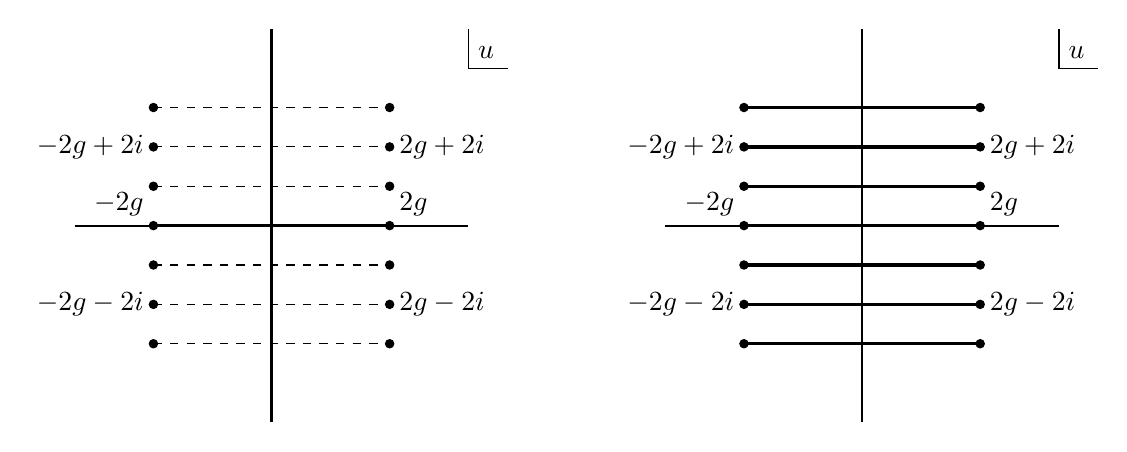
\begin{tikzpicture}[scale=0.5]
	
	%\draw[help lines] (0,0) grid (30,15);
	
	\tikzset{pole/.style={draw,circle,inner sep=0pt,minimum size=3pt,fill=black}}
	
	% P cuts
	
	\begin{scope}[shift={(6,6)}]
	
		\draw (5,5) -- (5,4) -- (6,4); \node[above right] at (5,4) {$u$};
	
		\draw[thick] (-5,0) -- (5,0); 
		\draw[thick] (0,-5) -- (0,5);
		
		\def\cutx{3}
		
		\foreach \y in {1,2,3} {
			\draw[dashed,black] (-\cutx,-\y) -- (\cutx,-\y);  
			\node[pole] at (-\cutx,-\y) {}; %\node[below left] at (-\cutx,-\y) {$-2g-\y i$};
			\node[pole] at (\cutx,-\y) {}; %\node[below right] at (\cutx,-\y) {$2g-\y i$};
			
			
			\draw[dashed,black] (-\cutx,\y) -- (\cutx,\y);  
			\node[pole] at (-\cutx,\y) {}; %\node[above left] at (-\cutx,\y) {$-2g+\y i$};
			\node[pole] at (\cutx,\y) {}; %\node[above right] at (\cutx,\y) {$2g+\y i$};
		}
		
		\draw[black,very thick] (-\cutx,0) -- (\cutx,0);  \node[pole] at (-\cutx,0) {}; \node[pole] at (\cutx,0) {};

		\node[above left] at (-\cutx,0) {$-2g$}; \node[above right] at (\cutx,0) {$2g$};	
		\node[left] at (-\cutx,-2) {$-2g-2 i$}; \node[right] at (\cutx,-2) {$2g-2 i$};		
		\node[left] at (-\cutx,2) {$-2g+2 i$}; \node[right] at (\cutx,2) {$2g+2 i$};	
	
	\end{scope}
	
	% \mu cuts
	
	\begin{scope}[shift={(21,6)}]
	
		\draw (5,5) -- (5,4) -- (6,4); \node[above right] at (5,4) {$u$};
		
		\draw[thick] (-5,0) -- (5,0); 
		\draw[thick] (0,-5) -- (0,5);
		
		\def\cutx{3}
		
		\foreach \y in {1,2,3} {
			\draw[black,very thick] (-\cutx,-\y) -- (\cutx,-\y);  
			\node[pole] at (-\cutx,-\y) {};
			\node[pole] at (\cutx,-\y) {};
			
			
			\draw[black,very thick] (-\cutx,\y) -- (\cutx,\y);  
			\node[pole] at (-\cutx,\y) {}; 
			\node[pole] at (\cutx,\y) {};
		}
		
		\draw[black,very thick] (-\cutx,0) -- (\cutx,0);  \node[pole] at (-\cutx,0) {}; \node[pole] at (\cutx,0) {};

		\node[above left] at (-\cutx,0) {$-2g$}; \node[above right] at (\cutx,0) {$2g$};	
		\node[left] at (-\cutx,-2) {$-2g-2 i$}; \node[right] at (\cutx,-2) {$2g-2 i$};		
		\node[left] at (-\cutx,2) {$-2g+2 i$}; \node[right] at (\cutx,2) {$2g+2 i$};

	
	\end{scope}
	
\end{tikzpicture}
\caption{The location of branch cuts in $u$ for the functions $\bP_a(u)$ (left) and $\hat{\mu}_{ab}(u)$ (right). The infinitely many cuts of $\tilde{\bP}_a$ are shown on the left picture with dashed lines.}
\label{fig:pmu_cuts}
\end{figure}
The magic of the whole quantum spectral curve construction is that the analytic continuations of the monodromies $\mu_{ab}$ through the cuts are again given by the same functions \cite{Gromov:2014caa}
\beq
	\label{muPPt-eq}
	\tilde\mu_{ab}-\mu_{ab}=\bP_a\tilde \bP_b-\bP_b\tilde \bP_a\;
\eeq
and the $\pmu$-system of eight $\bP$ and five $\mu$ functions closes!
The cut structure is shown in figure \ref{fig:pmu_cuts}.
An analogous closure can be implemented for the $\bQ$ functions by denoting the analytic continuations
\begin{equation}
\label{omegaQ}
\tilde \bQ_i=\omega_{ij} \bQ^j,
\end{equation}
where the monodromy $\omega$ is related to $\mu$ by
\beq
\label{muomega}
\omega_{ij}= \tilde{Q}_{a|i}^- \tilde{Q}_{b|j}^-\, \mu^{ab} \,.
\eeq
and itself has the following analytic continuation 
\begin{equation}\label{tQ=omegaQ}
\tilde\omega_{ij}-\omega_{ij}=\bQ_i\tilde{\bQ}_j-\bQ_j\tilde{\bQ}_i
\end{equation}
thus closing the $\bQ\omega$-system.
Both the $\pmu$ and the $\bQ\omega$-systems are complete in the sense they describe all solutions in the theory. 
Since they are related it is a matter of convenience to use one or the other and for the remainder of the thesis we will stick with the $\pmu$-system.

\subsubsection{Asymptotics}

Tracing back from the $\mathcal{Q}$-system to the Y-system one can find the following relation
\beq
	\label{eq:y_asymp}
	Y_{11} Y_{22} = 1 + \frac{\bP_1 \tilde{\bP_2} - \bP_2 \tilde{\bP_1}}{\mu_{12}} = \frac{\mu_{12}(u+i)}{\mu_{12}(u)}
\eeq
and thus given a solution to the $\pmu$-system one can fully reconstruct all of the Y-functions using the Y-system equations \eq{eq:ysystem}.
The Y-functions encode the global charges in their asymptotics, for example in the $\alg{sl}{2}$ sector one has \cite{Gromov:2011cx} 
\beq
	\label{eq:y1122_sl2_asymptotics}
	\log Y_{11} Y_{22} \; \simeq \; i \frac{\Delta - J}{u},
\eeq
implying through \eq{eq:y_asymp} that the asymptotics of the $\bP$ and $\mu$ functions also encode the global charges of the state/operator being described.

The picture described so far strongly resembles the classical spectral curve construction outlined in section \ref{sec:spectral_curve}.
Quite expectedly the classical spectral curve turns out to be the strong coupling limit of the quantum spectral curve as implied by the naming \cite{Gromov:2014caa}.
More precisely one can think of the classical spectral curve as an WKB approximation to the quantum case, namely the quasi-momenta are related to the $\bP$ and $\bQ$ functions as
\beq
	\bP_i \simeq e^{i\int^u \tilde{p}_i(u) \, du}, \;\;\; \bQ_i \simeq e^{i\int^u \hat{p}_i(u) \, du}
\eeq
where the four $\bP_i$ functions correspond to the $S^5$ momenta and the four $\bQ_i$ functions to the $AdS_5$ part.
The emergence of the cuts can be seen by recalling that the quasi-momenta are the eigenvalues of the monodromy matrix \eq{eq:lax_monodromy}, which develops the cuts after changing variables from $x$ to $u$ via the Zhukovsky map
\beq
	x + \frac{1}{x} = \frac{u}{g},
\eeq
which is the classical analogue of the rapidity map \eq{eq:xox_rapidity} from the asymptotic Bethe ansatz.
Similarly how the classical quasi-momenta encoded the global charges in their asymptotics as shown in \eq{eq:quasi_asymptotics}, so do their quantum analogues $\bP$ \cite{Gromov:2014caa}
\vspace{5pt}
\beq
\label{eq:pmu_large_u}
\left(
\bea{c}
\bP_1\\
\bP_2\\
\bP_3\\
\bP_4
\eea
\right)\simeq
\left(
\bea{l}
A_1\; u^\frac{-J_1-J_2+J_3-2}{2}\\
A_2\; u^\frac{-J_1+J_2-J_3}{2}\\
A_3\; u^\frac{+J_1-J_2-J_3-2}{2}\\
A_4\; u^\frac{+J_1+J_2+J_3}{2}
\eea
\right)\;\;,\;\;
\left(
\bea{c}
\bP^1\\
\bP^2\\
\bP^3\\
\bP^4
\eea
\right)\simeq
\left(
\bea{l}
A^1\; u^\frac{+J_1+J_2-J_3}{2}\\
A^2\; u^\frac{+J_1-J_2+J_3-2}{2}\\
A^3\; u^\frac{-J_1+J_2+J_3}{2}\\
A^4\; u^\frac{-J_1-J_2-J_3-2}{2}
\eea
\right)\; \vspace{3pt}
\eeq
and similarly for $\bQ$
\vspace{3pt}
\beq
\left(
\bea{c}
\bQ_1\\
\bQ_2\\
\bQ_3\\
\bQ_4
\eea
\right)\simeq
\left(
\bea{l}
B_1\; u^\frac{+\Delta-S_1-S_2}{2}\\
B_2\; u^\frac{+\Delta+S_1+S_2-2}{2}\\
B_3\; u^\frac{-\Delta-S_1+S_2}{2}\\
B_4\; u^\frac{-\Delta+S_1-S_2-2}{2}
\eea
\right)\;\;,\;\;
\left(
\bea{c}
\bQ^1\\
\bQ^2\\
\bQ^3\\
\bQ^4
\eea
\right)\simeq
\left(
\bea{l}
B^1\; u^\frac{-\Delta+S_1+S_2-2}{2}\\
B^2\; u^\frac{-\Delta-S_1-S_2}{2}\\
B^3\; u^\frac{+\Delta+S_1-S_2-2}{2}\\
B^4\; u^\frac{+\Delta-S_1+S_2}{2}
\eea
\right).\vspace{5pt}
\eeq
Since the $\pmu$ and $\bQ\omega$-systems are coupled via the QQ-relations the above asymptotics have to be compatible thus producing algebraic relations between the coefficients $A$ and the global charges.
We will be using simplified relations for the solutions we will consider later, the most general case can be found in \cite{Gromov:2014caa}.


\subsection{Revisiting the slope function}
\label{sec:slope_pmu}

In section \ref{sec:slope_function_aba} we derived the slope function which is the leading small spin expansion coefficient of the anomalous dimension for the generalized Konishi operator in the $\alg{sl}{2}$ sector.
We used the asymptotic Bethe ansatz as the starting point of the derivation which is justified by the fact that finite size effect are irrelevant for the slope function.
In this section we will derive the slope function \eq{eq:slope_function} using the $\pmu$-system, which is not only more concise but also generalizes to next orders as we shall demonstrate in the next section when we derive the next coefficient in the small spin expansion, the curvature function.

\subsubsection{$\pmu$-system for the $\alg{sl}{2}$ sector}
\label{sec:pmu_sl2}

The first simplification we can employ is the fact that solutions in the $\alg{sl}{2}$ sector are symmetric under the left-right exchange of the Y-functions $Y_{a,s}=Y_{a,-s}$, which implies the following relations for the $\bP$ and $\bQ$ functions
\begin{eqnarray}
&&\bP^a=\chi^{ac} \bP_c,\qquad  \bQ^i=\chi^{ij} \bQ_j
\end{eqnarray}
and thus the analytic continuation for the $\pmu$-system reads
\beq
\tilde \bP_a=-\mu_{ab}\chi^{bc}\bP_c,\; \ \ \ \text{with}\;\ \ \chi^{ab}=\left(
            \begin{array}{cccc}
              0 & 0 & 0 & -1 \\
              0 & 0 & 1 & 0 \\
              0 & -1 & 0 & 0 \\
              1 & 0 & 0 & 0 \\
            \end{array}
          \right),
\label{eq:Pmu}
\eeq
and
\beq
\tilde \mu_{ab}-\mu_{ab}=\bP_a \tilde\bP_b-  \bP_b \tilde\bP_a\;.
\label{eq:mudisc}
\eeq
Explicitly the $\pmu$-system equations are now given by
\beqa
\label{eq:pmuexpanded1}
&&\tilde \bP_1= -\bP_3 \mu_{12}+\bP_2 \mu_{13}-\bP_1 \mu_{14} \\
&&\tilde \bP_2= -\bP_4 \mu_{12}\hspace{16mm}+\bP_2 \mu_{14}-\bP_1 \mu_{24} \\
&&\tilde \bP_3= \hspace{16mm}-\bP_4 \mu_{13}+\bP_3 \mu_{14}\hspace{16mm}-\bP_1 \mu_{34} \\
&&\tilde \bP_4= \hspace{16mm}\hspace{15.5mm}-\bP_4 \mu_{14}+\bP_3 \mu_{24}-\bP_2 \mu_{34}\;.
\label{eq:pmuexpanded}
\eeqa
The above equations ensure that the branch points of $\bP_a$ and $\mu_{ab}$ are of the square root type, i.e. $\tilde{\tilde{\bP}}_a=\bP_a$ and $\tilde{\tilde{\mu}}_{ab}=\mu_{ab}$.
Finally, we require that $\bP_a$ and $\mu_{ab}$ do not have any singularities except these branch points.
%\footnote{For odd values of $J$ the functions $\bP_a$ may have an additional branch point at infinity. However, it should cancel in any product of two $\bP_a$'s, and therefore it will not appear in any physically relevant quantity (see \cite{Gromov:2013pga}, \cite{Gromov:2014caa}). We will discuss some explicit examples in the text.}.

The large $u$ asymptotics for the $\bP_a$ functions are given by \eq{eq:pmu_large_u} and can be uniquely fixed for the $\mu_{ab}$ functions using the $\pmu$-system \eq{eq:Pmu}-\eq{eq:mudisc}.
For the $\alg{sl}{2}$ sector they are given by \cite{Gromov:2013pga}
\beq
\bP_a\sim(A_1u^{-J/2},A_2u^{-J/2-1},A_3u^{J/2},A_4u^{J/2-1})
\label{eq:asymptotics}
\eeq
\beq
	\(\mu_{12},\ \mu_{13},\ \mu_{14},\ \mu_{24},\ \mu_{34}\)\sim
	\(u^{\Delta-J},\ u^{\Delta+1},\ u^{\Delta},\ u^{\Delta-1},\ u^{\Delta+J}\)
\label{eq:muasymptotics}
\eeq
where $J$ is the twist of the gauge theory operator, and $\Delta$ is its conformal dimension. 
With these asymptotics, the equations \eq{eq:Pmu}-\eq{eq:mudisc} form a closed system which fixes $\bP_a$ and $\mu_{ab}$.
Lastly, the spin $S$ of the operator is related \cite{Gromov:2013pga} to the leading coefficients $A_a$ of the $\bP_a$ functions
\beqa
&&A_1 A_4=\frac{\((J+S-2)^2-\Delta^2\)\((J-S)^2-\Delta^2\)}{16 i J(J-1)} \label{AA1} \\
&&A_2 A_3=\frac{\((J-S+2)^2-\Delta^2\)\((J+S)^2-\Delta^2\)}{16 i J(J+1)} \label{AA2},
\eeqa
which as discussed in the last section comes from the compatibility condition of the asymptotics for the $\pmu$ and $\bQ\omega$-systems.

Additionally the simplified $\bP\mu$-system enjoys a symmetry preserving all of its essential features. 
It has the form of a linear transformation of $\bP_a$ and $\mu_{ab}$ which leaves the system \eq{eq:Pmu}-\eq{eq:mudisc} and the asymptotics \eq{eq:asymptotics}, \eq{eq:muasymptotics} invariant. 
Indeed, consider a general linear transformation $\bP_a'={R_a}^b \bP_b$ with a non-degenerate constant matrix $R$. In order to preserve the system \eq{eq:Pmu}, $\mu$ should
at the same time be transformed as
\beq
\mu'=-R \mu \chi R^{-1}\chi.
\label{gammaP}
\eeq
Such a transformation also preserves the form of \eq{eq:mudisc} if
\beq
R^T\chi R\chi=-1\;,
\label{eq:sxsx}
\eeq
which also automatically ensures antisymmetry of $\mu_{ab}$ and the constraints (\ref{constraint}), (\ref{constraint2}).
However in general this transformation will spoil the asymptotics of $\bP_a$.
These asymptotics are ordered as $|\bP_2|<|\bP_1|<|\bP_4|<|\bP_3|$, which implies that the matrix $R$ must have the following structure
 \beq
R=\left(
\begin{array}{cccc}
 * & * & 0 & 0 \\
 0 & * & 0 & 0 \\
 * & * & * & * \\
 * & * & 0 & * \\
\end{array}
\right).
\eeq
This matrix would of course be lower triangular if we ordered $\bP_a$ by their asymptotics.
The general form of $R$ which satisfies \eq{eq:sxsx} and does not spoil the asymptotics generates a 6-parametric transformation, which we will call a $\gamma$-transformation. 
The simplest \text{$\gamma$-transformation} is the following rescaling:
\beq
\bP_1 \to \alpha \, \bP_1,\;\;
\bP_2 \to \beta \, \bP_2,\;\;
\bP_3 \to 1/\beta \, \bP_3,\;\;
\bP_4 \to 1/\alpha \, \bP_4,\;\;
\label{eq:alphabeta}
\eeq
\beq
\mu_{12} \to \alpha\beta \, \mu_{12},\;\;
\mu_{13} \to \frac{\alpha}{\beta} \, \mu_{13},\;\;
\mu_{14} \to \mu_{14}\;\;,\;\;
\mu_{24} \to \frac{\beta}{\alpha}\,\mu_{24},\;\;
\mu_{34} \to \frac{1}{\alpha\beta}\,\mu_{34},\;\;
\eeq
with $\alpha,\beta$ being constants.
In all the solutions that we consider all functions $\bP_a$ turn out to be functions of definite parity, so it makes sense to consider $\gamma$-transformations which preserve parity. 
$\bP_1$ and $\bP_2$  always have opposite parity as one can see from from \eq{eq:asymptotics} and thus should not mix under such transformations, the same is true about $\bP_3$ and $\bP_4$. 
Thus depending on parity of $J$ the parity-preserving $\gamma$-transformations are either
\beqa
\label{gammatransform2}
&\bP_3\rightarrow\bP_3+\gamma_3\bP_2,\ \bP_4\rightarrow\bP_4+\gamma_2\bP_1,\\
\nn&\mu_{13}\rightarrow\mu_{13}+\gamma_3\mu_{12},\ \mu_{24}\rightarrow\mu_{24}-\gamma_2\mu_{12},\ \mu_{34}\rightarrow\mu_{34}+\gamma_3\mu_{24}-\gamma_2\mu_{13}-\gamma_2\gamma_3\mu_{12}
\eeqa
for odd $J$ or
\beqa
\label{gammatransform1}
&\bP_3\rightarrow\bP_3+\gamma_1\bP_1,\ \bP_4\rightarrow\bP_4-\gamma_1\bP_2,\\
\nn&\mu_{14}\rightarrow\mu_{14}-\gamma_1\mu_{12},\ \mu_{34}\rightarrow\mu_{34}+2\gamma_1\mu_{14}-\gamma^2_1\mu_{12}\;,
\eeqa
for even $J$.

\subsubsection{Solving the system}

The description of the $\bP\mu$-system in the previous section was done for physical operators with the charges $S$ and $J$ being integers. 
Our goal is to take some peculiar limit when the (integer) number of covariant derivatives $S$ goes to zero.  
As we will see this requires some extension of the asymptotic requirement for $\mu$ functions.
In this section we will be guided by principles of naturalness and simplicity to deduce these modifications which we will summarize in section~\ref{sec:ancont}. 
There we also give a concrete prescription for analytical continuation in $S$, which we then use to derive the curvature function.
We also note that the solution of the $\pmu$-system is a little simpler for even $J$, because for odd $J$ extra branch points at infinity will appear in $\bP_a$ due to the asymptotics \eq{eq:asymptotics}, thus we will start with the $J$ even case.

We start solving the $\pmu$-system by first finding $\mu_{ab}$. 
Recalling that $\Delta=J+{\cal O}(S)$, from \eq{AA1}, \eq{AA2} we see that $A_1A_4$ and $A_2A_3$ are of order $S$ for small $S$, so we can take the functions $\bP_a$ to be of order $\sqrt{S}$. 
This is a key simplification, because now \eq{eq:mudisc} indicates that the discontinuities of $\mu_{ab}$ on the cut are small when $S$ goes to zero. 
Thus at leading order in $S$ all $\mu_{ab}$ are just periodic entire functions without cuts.
For power-like asymptotics of $\mu_{ab}$ like in \eq{eq:muasymptotics} the only possibility is that they are all constants.
However, we found that in this case there is only a trivial solution, i.e. $\bP_a$ can only be zero.
The reason for this is that for physical states $S$ must be integer and thus cannot be arbitrarily small, nevertheless, it is a sensible question how to define an analytical continuation from integer values of $S$.
Restricting the large positive $S$ behaviour one can show uniqueness of the continuation.

Thus we have to relax the requirement of power-like behaviour at infinity. The first possibility is
to allow for $e^{2\pi u}$ asymptotics at $u\to +\infty$.
We should, however, remember about the constraints \eq{constraint} and \eq{constraint2} which restrict our choice and the fact that we can also use $\gamma$-symmetry.
Let us show that by allowing $\mu_{24}$ to have exponential behaviour and setting it to $\mu_{24}=C\sinh(2\pi u)$ we arrive to the correct result. 
We analyse the reason for this choice in detail in section~\ref{sec:ancont}.

To simplify the constant part of $\mu_{ab}$ let us now make use of the $\gamma$-transformation, described in the last subsection.
This allows us to set $\mu_{12}=1,\;\mu_{34}=0$ and the constant $C$ to $1$ then the constraint \eq{constraint} imposes $\mu_{13}=0$ and $\mu_{14}=-1$.
Having fixed all $\mu$'s at leading order we get the following system of equations for $\bP_a$:
\beqa
&&\tilde \bP_1= -\bP_3 +\bP_1, \label{eq:P1L2} \\
&&\tilde \bP_2= -\bP_4 -\bP_2 -\bP_1 \sinh(2\pi u), \label{eq:P2L2}\\
&&\tilde \bP_3= \hspace{10mm}-\bP_3,\hspace{16mm} \label{eq:P3L2} \\
&&\tilde \bP_4= \hspace{10mm}+\bP_4+\bP_3 \sinh(2\pi u).\label{eq:P4L2}
\eeqa
Recalling that the functions $\bP_a$ only have a single short cut, we see from these equations that $\tilde{\bP}_a$ also have only this cut! 
This means that we can take all $\bP_a$ to be infinite Laurent series in the Zhukovsky variable $x(u)$, which rationalizes the Riemann surface with two sheets and one cut. 
It is defined by the ubiquitous mapping
\beq
	x+\frac{1}{x}=\frac{u}{g}
\eeq
where we pick the solution with a short cut, i.e.
\beq
x(u)=\frac{1}{2}\left(\frac{u}{g}+\sqrt{\frac{u}{g}-2}\;\sqrt{\frac{u}{g}+2}\;\right)\;\;.\;\;
\eeq
Solving the equations \eq{eq:P1L2} and \eq{eq:P3L2} with the asymptotics \eq{eq:asymptotics} we uniquely fix $\bP_1=\epsilon \, x^{-J/2}$ and $\bP_3=\epsilon\(x^{-J/2}-x^{+J/2}\)$, where $\epsilon$ is a constant yet to be found which we expect to be proportional to $\sqrt{S}$.
Thus the equations \eq{eq:P2L2} and \eq{eq:P4L2} become
\beqa
\label{eq:P2eq}
\tilde \bP_2+\bP_2&=& -\bP_4 -\epsilon x^{-J/2}\sinh(2\pi u)\;, \\
\label{eq:P4eq}
\tilde \bP_4-\bP_4&=& \epsilon(x^{-J/2}-x^{+J/2}) \sinh(2\pi u)\;.
\eeqa
We will first solve the second equation.
It is useful to introduce operations $[f(x)]_+$ and $[f(x)]_-$, which take parts of Laurent series with positive and negative powers of $x$ respectively.  
Taking into account that
\beq
	\sinh(2\pi u)=\sum\limits_{n=-\infty}^{\infty}I_{2n+1}  x^{2n+1},
\eeq
where $I_k\equiv I_{k}(4 \pi g)$ is the modified Bessel function of the first kind, we can write $\sinh(2\pi u)$ as
\beq
 \sinh(2\pi u)= \sinh_++\sinh_-,
\eeq
 where explicitly
\beqa
&& \sinh_+=[\sinh(2\pi u)]_+=\sum\limits_{n=1}^\infty I_{2n-1}x^{2n-1} \\
\label{defshm}
&& \sinh_-=[\sinh(2\pi u)]_-=\sum\limits_{n=1}^\infty I_{2n-1}x^{-2n+1}\;.
\eeqa
We now take the following ansatz for $\bP_4$
\beq
\bP_4=\epsilon(x^{J/2}-x^{-J/2})\sinh_-+Q_{J/2-1}(u),
\eeq
where $Q_{J/2-1}$ is a polynomial of degree $J/2-1$ in $u$. 
It is easy to see that this ansatz solves \eq{eq:P4eq} and has correct asymptotics. 
The polynomial $Q_{J/2-1}$ can be fixed from the equation \eq{eq:P2eq} for $\bP_2$. 
Indeed, from the asymptotics of $\bP_2$ we see that the lhs of \eq{eq:P2eq} does not have powers of $x$ from $-J/2+1$ to $J/2-1$. 
This fixes
\beq
Q_{J/2-1}(x)=-\epsilon\sum\limits_{k=1}^{J/2}I_{2k-1}\(x^{\frac{J}{2}-2k+1}+x^{-\frac{J}{2}+2k-1}\).
\eeq
Once $Q_{J/2-1}$ is found, we set $\bP_2$ to be the part of the right hand side of \eq{eq:P2eq} with powers of $x$ less than $-J/2$, which gives
\beq
\bP_2=-\epsilon x^{+J/2} \sum_{n=\frac{J}{2}+1}^\infty I_{2n-1}x^{1-2n}.
\eeq
This completes the solution for even $J$, we summarize it below:
\beqa
\label{eq:musolLOevenL}
&&\mu_{12}=1,\ \mu_{13}=0,\ \mu_{14}=-1,\ \mu_{24}=\sinh(2\pi u),\ \mu_{34}=0,\\
\label{eq:P1solLOevenL}
&&\bP_1=\epsilon x^{-J/2}\\
\label{eq:P2solLOevenL}
&&\bP_2=-\epsilon x^{+J/2} \sum_{n={J/2}+1}^\infty I_{2n-1}x^{1-2n}\\
\label{eq:P3solLOevenL}
&&\bP_3=\epsilon \(x^{-J/2}-x^{+J/2}\)\\
\label{eq:P4solLOevenL}
&&
	\bP_4=\epsilon \(x^{J/2}-x^{-J/2}\)\sinh_- -\epsilon \sum\limits_{n=1}^{J/2}I_{2n-1}\(x^{\frac{J}{2}-2n+1}+x^{-\frac{J}{2}+2n-1}\)\;.
\label{solutionevenL}
\eeqa
In the next subsection we fix the remaining parameter $\epsilon$ of the solution in terms of $S$ and find the energy, but now
let us briefly discuss the solution for odd $J$. 
As we mentioned above the main difference is that the functions $\bP_a$ now have a branch point at $u=\infty$, which is dictated by the asymptotics \eq{eq:asymptotics}. 
In addition, the parity of $\mu_{ab}$ is different according to the asymptotics of these functions \eq{eq:muasymptotics}. 
The solution is still very similar to the even $J$ case, and we discuss it in detail in Appendix \ref{sec:oddL}. 
Let us present the result here:
\beq
	\mu_{12}=1,\ \mu_{13}=0,\ \mu_{14}=0,\  \mu_{24}=\cosh(2\pi u),\ \mu_{34}=1
\eeq
\beqa
\label{P1oddL}
&&   \bP_1=\epsilon  x^{-J/2}, \\
&&   \bP_2=-\epsilon  x^{J/2}\sum\limits_{k=-\infty}^{-\frac{J+1}{2}}I_{2k}x^{2k},\\
&&   \bP_3=-\epsilon  x^{J/2}, \\
\label{P4oddL}
&&    \bP_4=\epsilon  x^{-J/2}\cosh_--\epsilon  x^{-J/2}\sum\limits_{k=1}^{\frac{J-1}{2}}I_{2k}x^{2k}-\epsilon  I_0 x^{-J/2}.
\eeqa
Note that now $\bP_a$ include half-integer powers of $x$.

\subsubsection{Fixing the global charges of the solution.}
\label{sec:LOresultevenL}

Finally, to fix our solution completely we have to find the value of $\epsilon$ and find the energy in terms of the spin using \eq{AA1} and \eq{AA2}.
For this we first extract the coefficients $A_a$ of the leading terms for all $\bP_a$, c.f. \eq{eq:asymptotics}.
From \eq{eq:P1solLOevenL}-\eq{eq:P4solLOevenL} or \eq{P1oddL}-\eq{P4oddL}
we get
\beqa
\label{Aexp1}
&& A_1= g^{J/2} \epsilon , \\
&& A_2=-g^{J/2+1} \epsilon  I_{J+1}, \\
\label{eq:A3LOL3}
&& A_3=-g^{-J/2} \epsilon , \\
\label{Aexplast}
&& A_4=-g^{-J/2+1}\epsilon  I_{J-1}.
\eeqa
Expanding \eq{AA1}, \eq{AA2} at small $S$ with $\Delta=J+S+\gamma$, where $\gamma={\cal O}(S)$, we find at linear order
\beqa
&& \gamma=i(A_1 A_4-A_2 A_3) \\
&& S=i(A_1A_4+A_2A_3)\;.
\eeqa
Plugging in the coefficients \eq{Aexp1}-\eq{Aexplast} we find that
\beq
\label{epss}
	\epsilon=\sqrt{\frac{2\pi i S}{JI_J(\sqrt\lambda)}}
\eeq
and we obtain the anomalous dimension at leading order,
\beq
\gamma=\frac{\sqrt{\lambda}I_{J+1}(\sqrt{\lambda})}{JI_J(\sqrt{\lambda})}S+{\cal O}(S^2),
\label{eq:resultLO}
\eeq
where the leading coefficient is precisely the slope function \eq{eq:slope_function} for the mode number $n=1$.
In fact the above calculation can be easily generalized for higher mode numbers. 
In the asymptotic Bethe ansatz for such operators we have two symmetric cuts formed by Bethe roots, with corresponding mode numbers being $\pm n$ (for the ground state $n=1$). 
To describe these operators within the $\bP\mu$-system we found that we should take $\mu_{24}=C\sinh(2\pi n u)$ instead of $\mu_{24}=C\sinh(2\pi u)$ (and for odd $J$ we similarly use $\mu_{24}=C\cosh(2\pi n u)$ instead of $\mu_{24}=C\cosh(2\pi u)$). 
Then the solution is very similar to the one above, and we find
\beq
\gamma=\frac{n\sqrt{\lambda}I_{J+1}(n\sqrt{\lambda})}{JI_J(n\sqrt{\lambda})}S\;,
\label{slopen}
\eeq
which exactly reproduces \eq{eq:slope_function} with $\Lambda \equiv n \sqrt{\lambda}$. 
In Appendix \ref{sec:Sanyn} we also show how using the $\bP\mu$-system one can reproduce the slope function for a configuration of Bethe roots with arbitrary mode numbers and filling fractions.

\subsubsection{Prescription for analytical continuation}
\label{sec:ancont}

To deduce the general prescription for the asymptotics of $\mu_{ab}$ for non-integer $S$ from our analysis, we first study the possible asymptotics of $\mu_{ab}$ for given $\bP_a$ in more detail. 
For that we combine the periodicity constraint \eq{muper} with \eq{eq:Pmu} and \eq{eq:mudisc} to write a finite difference equation on $\mu_{ab}$,
\beq\label{5bax}
\mu_{ab}(u+i)=\mu_{ab}(u)-\mu_{bc}(u)\chi^{cd}\bP_d\bP_a+\mu_{ac}(u)\chi^{cd}\bP_d\bP_b.
\eeq
As there are $5$ linear independent components of $\mu_{ab}$ this is a 5th order finite-difference equation which has $5$ independent solutions which we denote $\mu_{ab,A},\;A=1,\dots,5$.
Given the asymptotics of $\bP_a$ in \eq{eq:asymptotics} and \eq{AA1}, \eq{AA2} there are exactly $5$ different asymptotics a solution of \eq{5bax} could have as discussed in \cite{Gromov:2013pga}.
We denote these $5$ independent solutions of \eq{5bax} as $\mu_{12,A}$ where $A=1,\dots,5$ and summarize their leading asymptotics at large $u>0$ in the table below
\beq
\bea{c||l|l|l|l|l}
A=&1&2&3&4&5\\ \hline\hline
\mu_{12,A}\sim & u^{\Delta-J}& C_{1,2} u^{-S+1-J}& C_{1,3} u^{-J}& C_{1,4} u^{S-1-J}& C_{1,5} u^{-\Delta-J}\\
\mu_{13,A}\sim & C_{2,1} u^{\Delta+1}& C_{2,2} u^{-S+2}& C_{2,3} u^{+1}& { u^{S}}& C_{2,5} u^{-\Delta+1}\\
\mu_{14,A}\sim & C_{3,1} u^{\Delta}& C_{3,2} u^{-S+1}& 1 & C_{3,4} u^{S-1}& C_{3,5} u^{-\Delta}\\
\mu_{24,A}\sim & C_{4,1} u^{\Delta-1}& u^{-S}& C_{4,3} u^{-1}& C_{4,4} u^{S-2}& C_{4,5} u^{-\Delta-1}\\
\mu_{34,A}\sim & C_{5,1} u^{\Delta+J}& C_{5,2} u^{-S+1+J}& C_{5,3} u^{+J}& C_{5,4} u^{S-1+J}& { u^{-\Delta+J}}
\label{tablemu}
\eea
\eeq
where we fix the normalization of our solutions so that some coefficients are set to $1$. 
The coefficients $C_{a,A}$ are some rational functions of $S,\Delta,J$ and $A_1,A_2$ and in the small $S$ limit all $C_{a,A}\to 0$ in our normalization.
As it was pointed out in \cite{Gromov:2013pga} the asymptotics for different $A's$ are obtained by replacing $\Delta$ in \eq{eq:muasymptotics} by $\pm \Delta,\pm (S-1) $ and $0$.
We label these solutions so that in the small $S$ regime these asymptotics are ordered $\Delta> 1-S>0>S-1>-\Delta$.
Of course any solution of \eq{5bax} multiplied by an $i$-periodic function will still remain a solution of \eq{5bax}.
The true $\mu_{ab}$ is thus a linear combination of the partial solutions $\mu_{ab,A}$ with some constant or periodic coefficients.
This particular combination should in addition satisfy the analyticity condition \eq{muper} which is not guaranteed by \eq{5bax}.

The prescription for analytical continuation in $S$ which we propose here is based on the large $u$ asymptotics of these periodic coefficients.
As we discussed in the previous section the assumption that all these coefficients are asymptotically constant is too constraining already at the leading order in $S$, and we must assume that at least some of these coefficients grow exponentially as $e^{2\pi u}$.
To get some extra insight into the asymptotic behaviour of these coefficients it is very instructive to go to the weak coupling regime.
It is known that at one loop the equation \eq{5bax} reduces to a second order equation. When written as a finite difference equation for $\mu_{12}$ it coincides exactly with the Baxter equation for the non-compact $\alg{sl}{2}$ spin chain. 
For $J=2$ it reads
\beq\label{oneloopbaxter}
\(2u^2-S^2-S-\frac{1}{2}\)Q(u)=(u+\tfrac{i}{2})^2 Q(u+i)
+(u-\tfrac{i}{2})^2 Q(u-i)
\eeq
where $Q(u)=\mu_{12}(u+i/2)$.
This equation is already very well studied and all its solutions are known explicitly \cite{Derkachov:2002wz} -- in particular it is easy to see that one of the solutions must have $u^S$ asymptotics at infinity, while the other behaves as $1/u^{S+1}$.
It is also known that at one loop and for any integer $S$ \eq{oneloopbaxter} has a polynomial solution which gives the energy as 
\beq
	\Delta=J+S+\left.2ig^2\d_u\log\frac{Q(u-i/2)}{Q(u-i/2)}\right|_{u=0}=S+J+8g^2 H_S.
\eeq
At the same time, for non-integer $S$ there are of course no polynomial solutions, and according to \cite{Janik:2013nqa} and \cite{Alfimov:2014bwa} the solution which produces the energy $S+J+8g^2 H_S$ cannot even have power-like asymptotics, instead the correct large $u$ behaviour must be
\beq
Q(u)\sim \(u^S+\dots\)+(A+B e^{2\pi u})\(\frac{1}{u^{S+1}}+\dots\)\;\;,\;\;u\to +\infty\;.
\eeq
Furthermore, there is a unique entire $Q$ function with the above asymptotics.
For $S>-1/2$ we can reformulate the prescription by saying that the correct solution has power-like asymptotics, containing all possible solutions, plus a small solution reinforced with an exponent.
In this form we can try to translate this result to our case. 
We notice that for $g\to 0$ we have $\mu_{12,1}\sim u^{S}$ and $\mu_{12,2}\sim u^{-S-1}$, which tells us that at least the second solution must be allowed to have a non-constant periodic coefficient in the asymptotics. 
We also assume that the coefficient in front of $\mu_{ab,3}$ tends to a constant\footnote{It could be hard or even impossible to separate $\mu_{ab,3}$ from $\mu_{ab,2}$ in a well defined way.
In these cases $\mu_{ab,2}$ is defined modulo $\mu_{ab,3}$ and other subleading solutions. 
Our prescription then means that the exponential part of the coefficient in front of $\mu_{ab,3}$ is proportional to that of in front of $\mu_{ab,2}$.}.
This extra condition does not follow from the one loop analysis we deduced from our solution.
We will show how this prescription produces the correct known result for the leading order in $S$.
From our analysis it is hard to make a definite statement about the behaviour of the periodic coefficients in front of $\mu_{12,4}$ and  $\mu_{12,5}$, but due to the expected $\Delta \to-\Delta$ symmetry, which interchanges $\mu_{12,5}$ and $\mu_{12,1}$, one may expect that the coefficient of $\mu_{12,5}$ should also go to a constant. 
To summarize we should have
\beq\label{prescr}
\mu_{ab}(u)=\sum_{A=1}^5 c_{A}\mu_{ab,A}(u)
+\sum_{A=2,4,5} p_{A}(u)\mu_{ab,A}(u)
\eeq
where $c_A$ are constants whereas $p_{A}(u)$ are some linear combinations of $e^{\pm 2\pi u}$\footnote{It could be that some of the coefficients of $p_{A}$ should be zero due to the constraint \eq{constraint}.}.

In the small $S$ limit, $\bP_a\to 0$ and the finite difference equation \eq{5bax} simply tells us that $\mu_{ab}(u+i)=\mu_{ab}(u)$ which implies that our $5$ independent solutions are just constants at the leading order in $S$.
We begin by noticing that in this limit $\mu_{12}$ must be entirely coming from $\mu_{12,1}$ as all the other solutions could only produce negative powers and thus cannot contribute at the leading order. 
So we start by imposing $\mu_{ab}=C_{ab}+D_{ab}\sinh(2\pi u)+E_{ab}\cosh(2\pi u)$ for some constants $C_{ab},D_{ab},E_{ab}$ such that $D_{12}=E_{12}=0$. 
Thus we have $5$ different $C$'s, $4$ different  $D$'s and $4$ different $E$'s.
We notice that this general form of $\mu_{ab}$ can be significantly simplified.
First, using the Pfaffian constraint \eqref{constraint} and the \text{$\gamma$-transformation} \eqref{gammaP} any generic $\mu_{ab}$ of this form can be reduced to one belonging to the following two-parametric family inside the original 13-parametric space
\beqa
&&\mu_{12}=1,\ \mu_{14}=a^2 \sinh{2\pi u}+\frac{a}{2}\cosh{2\pi u}\;,\\\
&&\mu_{24}=b\sinh{2\pi u}+\sinh{2\pi u}\;,\
\mu_{34}=\frac{a^2}{4}\frac{(1-2ab)^2}{b^2-1}+1\;,
\label{mufamilyab}
\eeqa
where $\mu_{13}$ is found from the Pfaffian constraint.
Second, recall that according to our prescription the 1st and 3rd solutions (columns in the table \eqref{tablemu}) cannot contain exponential terms.
Consider $\mu_{14}$ and $\mu_{24}$, we again see that the 4th and 5th solutions could only contain negative powers of $u$ and thus only the 2nd solution can contribute to the parts of $\mu_{14}$ and $\mu_{24}$ that are non-decaying at infinity.
This means that these components can be represented in the following form
\beqa
\mu_{14}=(a_1\sinh{2\pi u}+ a_2\cosh{2\pi u})\mu_{14,2}(u)+\mathcal{O}\(e^{2\pi u}/u\)\;,\\
\mu_{24}=(a_1\sinh{2\pi u}+a_2\cosh{2\pi u})\mu_{24,2}(u)+\mathcal{O}\(e^{2\pi u}/u\)\;,
\eeqa
for $u\to+\infty$.
The $\mathcal{O}\(e^{2\pi u}/u\)$ terms contain contributions from all of the solutions except for the 2nd. 
One can see that \eqref{mufamilyab} can be of this form only in two cases: if $a=0$ or if $a=\frac{1}{2b}$.
Both of these cases can be brought to the form
\beq
\label{muresan}
\mu_{12}=1,\ \mu_{13}=0,\ \mu_{14}=0,\ \mu_{24}=d_1\sinh{2\pi u}+d_2\cosh{2\pi u},\ \mu_{34}=1
\eeq
by a suitable $\gamma$-transformation \eqref{mufamilyab}. 
However, we found that there is an additional constraint which follows from compatibility of $\mu_{ab}$ with the decaying asymptotics of $\bP_2$. 
As we show in appendix \ref{sec:Sanyn} for even $J$ one must set $d_2=0$. 
For odd $J$ we must set $d_1=0$ as a compatibility requirement. 
This justifies the choice of $\mu_{ab}$ used in the previous section.
In the next section we will show how the same prescription can be applied at the next order in $S$ and leads to non-trivial results which we subjected to intensive tests later in the text.

\subsection{The curvature function}
\label{sec:curvature}

In this section we use the $\bP\mu$-system to compute the next coefficient in the small spin expansion of the folded string solution after the slope, which we call the curvature function $\gamma^{(2)}(g)$. 
First we will discuss the case $J=2$ in detail and then describe the modifications of the solution for the cases $J=3$ and $J=4$, more details on which can be found in appendix \ref{sec:NLOapp}.

% \subsubsection{Iterative procedure for the small $S$ expansion of the $\bP\mu$-system}
% \label{sec:SolvingPmuL2}

For convenience let us repeat the leading order solution \eq{eq:musolLOevenL}-\eq{eq:P4solLOevenL} of the $\bP\mu$-system for the slope function in the case when $J=2$
\beqa
{\bf P}^{(0)}_1=\epsilon\frac{1}{x}\;\;&,&\;\;{\bf P}^{(0)}_2=+\epsilon I_1-\epsilon x[\sinh(2\pi u)]_-\;\;,\\
{\bf P}^{(0)}_3=\epsilon\(\frac{1}{x}-x\)\;\;&,&\;\;
{\bf P}^{(0)}_4=
-2\epsilon I_1-
\epsilon \(\frac{1}{x}-x\)[\sinh(2\pi u)]_-.
\label{P10P40}
\eeqa
Here $\epsilon$ is a small parameter, proportional to $\sqrt{S}$ as seen in \eq{epss} and by $\bP_a^{^{(0)}}$ we denote the $\bP_a$ functions at leading order in $\epsilon$.
The key observation is that the $\bP\mu$-system can be solved iteratively order by order in $\epsilon$. 
Let us write $\bP_a$ and $\mu_{ab}$ as an expansion in this small parameter
\beq
	\bP_a=\epsilon\bP_a^{(0)}+\epsilon^3\bP_a^{(1)}+\epsilon^5\bP_a^{(2)}+\dots
\eeq
\beq
	\mu_{ab}=\mu_{ab}^{(0)}+\epsilon^2\mu_{ab}^{(1)}+\epsilon^4\mu_{ab}^{(2)}+\dots \;.
\eeq
This structure of the expansion is dictated by the equations \eq{eq:Pmu} and \eq{eq:mudisc} of the $\bP\mu$-system as we will soon see explicitly. 
Since the leading order $\bP_a$ are of order $\epsilon$, equation \eq{eq:mudisc} implies that the discontinuity of $\mu_{ab}$ on the cut is of order $\epsilon^2$. 
Thus to find $\mu_{ab}$ in the next to leading order (NLO) we only need the functions $\bP_a$ at leading order. 
After this, we can find the NLO correction to $\bP_a$ from equations \eq{eq:mudisc}. 
This will be done below, and having thus the full solution of the $\bP\mu$-system at NLO we will find the energy at order $S^2$.

\subsubsection{Correcting $\mu_{ab}$}
\label{sec:muNLOL2}
In this subsection we find the NLO corrections $\mu^{(1)}_{ab}$ to $\mu_{ab}$. 
As follows from \eq{eq:mudisc} and \eq{muper} they should satisfy the equation
\beq
 \mu_{ab}^{(1)}(u+i)-\mu_{ab}^{(1)}(u)=\bP_a^{(0)} \tilde\bP_b^{(0)}-  \bP_b^{(0)} \tilde\bP_a^{(0)},
\label{eq:mudiscNLO}
\eeq
in which the right hand is known explicitly. 
For that reason let us define an apparatus for solving equations of this type, i.e.
\beq
f(u+i)-f(u)=h(u).
\label{eqperiod}
\eeq
More precisely, we consider functions $f(u)$ and $h(u)$ with one cut in $u$ between $-2g$ and $2g$, and no poles. 
Such functions can be represented as infinite Laurent series in the Zhukovsky variable $x(u)$, and we additionally restrict ourselves to the case where for $h(u)$ this expansion does not have a constant term\footnote{The r.h.s. of \eq{eq:mudiscNLO} has the form $F(u)-\tilde F(u)$ and therefore indeed does not have a constant term in its expansion, as the constant in $F$ would cancel in the difference $F(u)-\tilde F(u)$.}.
One can see that the general solution of \eq{eqperiod} has a form of a particular solution plus an arbitrary $i$-periodic function, which we also call a zero mode. 
% The class of $i$-periodic function we consider here is restricted to $\sinh(2\pi u)$, $\cosh(2\pi u)$ and constants (for discussion of higher modes $\sinh(2\pi n u), \cosh(2\pi n u)$ see appendix \ref{sec:appHigher}).
First we will describe the construction of the particular solution and later deal with zero modes. 

The linear operator which gives the particular solution of \eq{eqperiod} described below will be denoted as $\Sigma$.
Notice that given the explicit form \eq{P10P40} of $\bP^{(0)}_a$, the right hand side of \eq{eq:mudiscNLO} can be represented in a form
\beq
\alpha(x)\sinh(2\pi u)+\beta(x),
\label{alphabetasinh}
\eeq
where $\alpha(x),\beta(x)$ are power series in $x$ growing at infinity not faster than polynomially. 
Thus for such $\alpha$ and $\beta$ we define
\beq
\Sigma\cdot\[\alpha(x)\sinh(2\pi u)+\beta(x)\]\equiv \sinh(2\pi u) \Sigma\cdot \alpha(x)+\Sigma\cdot \beta(x).
\eeq
We also define $\Sigma\cdot x^{-n}=\Gamma'\cdot x^{-n}$ for $n>0$, where the integral operator $\Gamma'$ defined as
\beq
\(\Gamma'\cdot h\)(u)\equiv \oint_{-2g}^{2g}\frac{dv}{{4\pi i}}\partial_u \log \frac{\Gamma[i (u-v)+1]}{\Gamma[-i (u-v)]}h(v).
\label{Gammaprime}
\eeq
This requirement is consistent because of the following relation\footnote{We remind that $f_+$ and $f_-$ stand for the part of the Laurent expansion with, respectively, positive and negative powers of $x$, while $\tilde f$ is the analytic continuation around the branch point at $u=2g$ (which amounts to replacing $x\to\frac{1}{x}$)}
\beq
\(\Gamma'\cdot h\)(u+i)-\(\Gamma'\cdot h\)(u)
=
-\frac{1}{2\pi i}\oint_{-2g}^{2g}\frac{h(v)}{u-v}dv=h_-(u)-\widetilde{h_+}(u).
\label{eq:Gammaproperty}
\eeq
What is left is to define $\Sigma$ on positive powers of $x$. 
We do it by requiring
\beq
\Sigma\cdot\left[x^a+1/x^a\right]\equiv p_a'(u) %=2 \Sigma\cdot\left[T_a\(\frac{u}{2g}\)\right],
\label{paprime}
\eeq
where $p_a'(u)$ is a polynomial in $u$ of degree $a+1$, which is a solution of
\beq
p_a'(u+i)-p_a'(u)=\frac{1}{2}\(x^a+1/x^a\)
\eeq
and satisfies the following additional properties: $p_a'(0)=0$ for odd $a$  and $p_a'(i/2)=0$ for even $a$. 
One can check that this definition is consistent and defines of $p'_a(u)$ uniquely. 
Explicit form of the first few $p_a'(u)$, which we call periodized  Chebyshev polynomials, can be found in appendix \ref{sec:appPeriodized}.
%where $T_a(u)$ are Chebyshev polynomials of the first kind.
From this definition of $\Sigma$ one can see that the result of its action on expressions of the form \eq{alphabetasinh} can again be represented in this form - what is important for us is that no exponential functions other than $\sinh(2\pi u)$ appear in the result.

A good illustration of how the definitions above work would be the following two simple examples.
Suppose one wants to calculate $\Sigma\cdot\(x-\frac{1}{x}\)$, then it is convenient to split the argument of $\Sigma$ in the following way:
\beq
\Sigma\cdot\(x-\frac{1}{x}\)=\Sigma\cdot\(x+\frac{1}{x}\)-2\,\Sigma\cdot\frac{1}{x}.
\eeq
In the first term we recognize $p_1'(u)=\frac{i u(u-i)}{2g}$, whereas in the second the argument of $\Sigma$ is decaying at infinity, thus $\Sigma$ is equivalent to $\Gamma'$ in this context. 
Notice also that $\Gamma'\cdot \frac{1}{x}=-\Gamma'\cdot x$. 
All together we get
\beq
\Sigma\cdot\(x-\frac{1}{x}\)=\Sigma\cdot\(x+\frac{1}{x}\)-2\,\Sigma\cdot\frac{1}{x}=2\,p_1'(u)+ 2 \,\Gamma'\cdot x.
\eeq
In a similar way, in order to calculate $\Sigma\cdot \(\sinh_--\sinh_+\) / 2$, one can write 
\beq
	\frac{\sinh_--\sinh_+}{2}=\sinh_- \, - \, \frac{1}{2}\sinh(2\pi u).
\eeq
Notice that since $\sinh_-$ decays at infinity, thus
\beq
\Sigma\cdot\sinh_-=\Gamma'\cdot\sinh_-.
\eeq
 Also, since $i$-periodic functions can be factored out of $\Sigma$,
\beq
\Sigma\cdot\sinh(2\pi u)=\sinh(2\pi u)\Sigma\cdot 1=\sinh(2\pi u)p_0'(u)/2.
\eeq
Finally,
\beq
\Sigma\cdot\frac{\sinh_--\sinh_+}{2}=\Gamma'\cdot(\sinh_-)-\frac{1}{2}\sinh(2\pi u)p_0'(u).
\eeq
As an example we present the particular solution for two components of $\mu_{ab}$.
\beqa
\label{muexpl1}
\mu_{13}^{(1)}-\pi_{13}&=&\Sigma\cdot\({\bf P}_1 \tilde{\bf P}_3-{\bf P}_3 \tilde{\bf P}_1\)=\epsilon^2\,\Sigma\cdot\(x^2-\frac{1}{x^2}\) =\epsilon^2\;\(\Gamma'\cdot x^2+p_2'(u)\),\\
\nonumber
\mu_{12}^{(1)}-\pi_{12}&=&\Sigma\cdot\({\bf P}_1
   \tilde{\bf P}_2-{\bf P}_2
   \tilde{\bf P}_1\)= \\ &=&
   -\epsilon^2\[2 I_1\Gamma'\cdot x-\sinh(2\pi u)\;\Gamma'\cdot x^2-\Gamma'\cdot\(\sinh_-\(x^2+\frac{1}{x^2}\)\)
   \].\;\;\;\;\;\;\;\qquad\label{muexpl2}
\eeqa
Below we will argue that $\pi_{12}$ and $\pi_{13}$ can be chosen to be zero, as seen in \eq{eq:periodicpart}.
Now let us apply $\Sigma$ defined above to \eq{eq:mudiscNLO}, writing that its general solution is
\beq
\mu^{(1)}_{ab}=\Sigma\cdot(\bP_a^{(0)} \tilde\bP_b^{(0)}-  \bP_b^{(0)} \tilde\bP_a^{(0)})+\pi_{ab},
\label{eq:sol13}
\eeq
where the zero mode $\pi_{ab}$ is an arbitrary $i$-periodic entire function, which can be written similarly to the leading order as $c_{1,ab}\cosh{2\pi u}+c_{2,ab}\sinh{2\pi u}+c_{3,ab}$. 
Again, many of the coefficients $c_{i,ab}$ can be set to zero. 
First, the prescription from section \ref{sec:ancont} implies that non-vanishing at infinity part of coefficients of $\sinh(2\pi u)$ and $\cosh(2\pi u)$ in $\mu_{12}$ is zero. 
As one can see from the explicit form \eq{muexpl2} of the particular solution which we choose for $\mu_{12}$, it does not contain $\cosh(2\pi u)$ and the coefficient of $\sinh(2\pi u)$ is decaying at infinity. 
So in order to satisfy the prescription, we have to set $c_{2,12}$ and $c_{2,12}$ to zero. 
Second, since the coefficients $c_{n,ab}$ are of order $S$, we can remove some of them by making an infinitesimal  $\gamma$-transformation with $R=1 + {\cal O}(S)$ in \eq{gammaP}.
Furthermore, the Pfaffian constraint \eq{constraint} imposes 5 equations on the remaining coefficients, which leaves the following 2-parametric family of zero modes
\beqa
\pi_{12}= \pi_{13} = 0,&&\ \pi_{14}=\frac{1}{2}c_{1,34}\cosh{2\pi u},\\
\pi_{24}= c_{1,24}\cosh{2\pi u},&&\ \pi_{34}= c_{1,34}\cosh{2\pi u}.
\eeqa
Let us now look closer at the exponential part of $\mu_{14}$ and $\mu_{24}$. 
Combining the leading order \eq{eq:musolLOevenL} and the perturbation \eq{eq:sol13} and taking into account the fact that operator $\Sigma$ does not produce terms proportional to $\cosh{2 \pi u}$, we obtain
\beqa
&&\mu_{14}=\frac{1}{2}c_{1,34}\cosh{2\pi u}+{\cal O}(\epsilon) \sinh{2\pi u}+\mathcal{O}(\epsilon^2)+\dots, \\
&&\mu_{24}=\frac{1}{2}c_{1,24}\cosh{2\pi u}+(1+{\cal O}(\epsilon)) \sinh{2\pi u}+\mathcal{O}(\epsilon^2)+\dots,
\eeqa
where dots stand for powers-like terms or exponential terms suppressed by powers of $u$.
As we remember from section \ref{sec:ancont}, only the 2nd solution of the 5th order Baxter equation \eq{5bax} can contribute to the exponential part of $\mu_{14}$ and $\mu_{24}$, which means that $\mu_{14}$ and $\mu_{24}$ are proportional to the same linear combination of $\sinh{2\pi u}$ and $\cosh{2\pi u}$. 
From the second equation one can see that this linear combination can be normalized to be $\frac{1}{2}c_{1,24}\cosh{2\pi u}+(1+{\cal O}(\epsilon)) \sinh{2\pi u}$ and thus 
\beq
	\mu_{14}=C\(\frac{1}{2}c_{1,24}\cosh{2\pi u}+(1+{\cal O}(\epsilon)) \sinh{2\pi u}\),
\eeq 
where $C$ is some constant, which is of order ${\cal O}(\epsilon)$, because the coefficient of $\sinh{2\pi u}$ in the first equation is ${\cal O}(\epsilon)$.
Taking into account that $c_{1,24}$ is ${\cal O}(\epsilon)$ itself, we find that $c_{1,34}=\mathcal{O}(\epsilon^2)$, i.e. it does not contribute at the order which we are considering. 
So the final form of the zero mode in \eq{eq:sol13} is
\beq
	\pi_{12} = \pi_{13} = \pi_{14} = \pi_{34}=0, \;\;\; \pi_{24}=c_{1,24}\cosh{2\pi u}.
	\label{eq:periodicpart}
\eeq
%The result of acting with $\Sigma$ on the combination $\bP_a^{(0)} \tilde\bP_b^{(0)}$ appearing in \eq{eq:sol13} can be %rewritten in terms of $\Gamma'$ and periodized versions of Chebyshev polynomials $p_a'(u)$ defined as
%\beq
%p_a'(u)=\Sigma\cdot\left[x^a+1/x^a\right]=2 \Sigma\cdot\left[T_a\(\frac{u}{2g}\)\right],
%\label{paprime}
%\eeq
%where $T_a(u)$ are Chebyshev polynomials of the first kind.
In this way, using the particular solution given by $\Sigma$ and the form of zero modes \eq{eq:periodicpart} we have computed all the functions $\mu_{ab}^{(1)}$. 
The details and the results of the calculation can be found in appendix \ref{sec:appmu2}.


\subsubsection{Correcting $\bP_{a}$}
\label{sec:CalculationofPa}

Now that we found the NLO part of $\mu_{ab}$ we can use the iterative procedure described at the beginning of the section to write a closed system of equations for $\bP_a^{(1)}$.
Indeed, expanding the system \eq{eq:pmuexpanded} to NLO we get
\beqa
\label{eq:P1eqNLOL2}
&&\tilde \bP^{(1)}_1
- \bP^{(1)}_1
= -\bP^{(1)}_3+r_1,  \\
\label{eq:P2eqNLOL2}
&&\tilde \bP^{(1)}_2+\bP_2^{(1)}= -\bP^{(1)}_4  -\bP^{(1)}_1 \sinh(2\pi u)+r_2, \\
\label{eq:P3eqNLOL2}
&&\tilde \bP^{(1)}_3+\bP_3^{(1)}=r_3,\\
\label{eq:P4eqNLOL2}
&&\tilde \bP^{(1)}_4-\bP_4^{(1)}=\bP_3^{(1)} \sinh(2\pi u)+r_4,
\eeqa
where the free terms are given by
\beq
r_a=-\mu_{ab}^{(1)}\chi^{bc}\bP_c^{(0)}.
\label{eq:ra}
\eeq
Notice that $r_a$ does not change if we add a matrix proportional to $\bP_a^{(0)} \tilde\bP_b^{(0)}-  \bP_b^{(0)} \tilde\bP_a^{(0)}$ to $\mu^{(1)}_{ab}$ due to the relations
\beq
	\bP_a \chi^{ab}\bP_b=0,\;\bP_a\chi^{ab}\tilde\bP_b=0,
\eeq	
which follow from the $\bP\mu$-system equations. 
In particular we can use this property to do the following replacement in \eq{eq:ra}
\beq
	\mu_{ab}^{(1)} \to \mu_{ab}^{(1)}+\frac{1}{2}\(\bP_a^{(0)} \tilde\bP_b^{(0)}-  \bP_b^{(0)} \tilde\bP_a^{(0)}\).
\eeq	
This will be convenient for us, since in expressions for $\mu^{(1)}_{ab}$ in terms of $p_a$ and $\Gamma$  as seen in \eq{muexpl1}, \eq{muexpl2} and appendix \ref{sec:appmu2}, this change amounts to simply replacing $\Gamma'$ by a convolution with a more symmetric kernel $\Gamma' \rightarrow  \Gamma$ defined by
\beq
\(\Gamma\cdot h\)(u)\equiv \oint_{-2g}^{2g}\frac{dv}{{4\pi i}}\partial_u \log \frac{\Gamma[i (u-v)+1]}{\Gamma[-i (u-v)+1]}h(v),
\label{Gamma}
\eeq
while at the same time replacing
\beq
	 p_a'(u)\rightarrow  p_a(u) = p_a'(u)+\frac{1}{2}\(x^a(u)+x^{-a}(u)\).
\label{pa}
\eeq


Having made this comment, we will now develop tools for solving the equations \eq{eq:P1eqNLOL2} - \eq{eq:P4eqNLOL2}.
Notice first that if we solve them in the order \eq{eq:P3eqNLOL2}, \eq{eq:P1eqNLOL2}, \eq{eq:P4eqNLOL2}, \eq{eq:P2eqNLOL2}, substituting into each subsequent equation the solution of all the previous, then at each step the problem we have to solve has a form
\beq
 \tilde f+f=h\;\; \text{or}\;\; \tilde f-f=h\;\;,
 \label{eq:eqs}
\eeq
where $h$ is known, $f$ is unknown and both the right hand side and the left hand side are power series in $x$. 
It is obvious that equations \eq{eq:eqs} have solutions only for $h$ such that $h=\tilde h$ and $h=-\tilde h$ respectively.
On the class of such $h$ a particular solution for $f$ can be written as
\beq
f= [h]_-+[h]_0/2\equiv H\cdot h\;\; \Rightarrow\;\; \tilde f+f=h
\label{eq:solfh1}
\eeq
and
\beq
f= [h]_-\equiv K\cdot h\;\; \Rightarrow\;\; \tilde f-f=h,
\label{eq:solfh2}
\eeq
where $[h]_0$ is the constant part of Laurent expansion of $h$ (it does not appear in the second equation, because $h$ such that $h=-\tilde h$ does not have a constant part).
The operators $K$ and $H$ introduced here can be also defined by their integral kernels
\beqa
H(u,v)&=&-\frac{1}{4\pi i}\frac{\sqrt{u-2g}\sqrt{u+2g}}{\sqrt{v-2g}\sqrt{v+2g}}\frac{1}{u-v}, \\
K(u,v)&=&+\frac{1}{4\pi i}\frac{1}{u-v},
\label{eq:HK}
\eeqa
which are equivalent to \eq{eq:solfh1}, \eq{eq:solfh2} of the classes of $h$ such that $h=\tilde h$ and $h=-\tilde h$ respectively.
%\footnote{We denote e.g. $K\cdot h=\oint_{-2g}^{2g}K(u,v)h(v)dv$ where the integral is around the branch cut between $-2g$ and $2g$.}. 
The particular solution $f=K\cdot h$ of the equation $\tilde f+ f=h$ is unique in the class of functions $f$ decaying at infinity, and the solution $f=H \cdot h$ of $\tilde f- f=h$ is unique for non-growing $f$. 
In all other cases the general solution will include zero modes, which, in our case are fixed by asymptotics of $\bP_a$.
Now it is easy to write the explicit solution of the equations
\eq{eq:P1eqNLOL2}-\eq{eq:P4eqNLOL2}:
\beqa
\bP_3^{(1)}&=&H\cdot r_3,\\
\bP_1^{(1)}&=&\frac{1}{2}\,\bP^{(1)}_3+K\cdot \(r_1-\frac{1}{2} r_3\),\\
\bP_4^{(1)}&=&K\cdot\(-\frac{1}{2}\(\tilde\bP_3^{(1)}-\bP_3^{(1)}\) \sinh(2\pi u)+
\frac{2r_4+r_3 \sinh(2\pi u)}{2}\)-2\,\delta,\;\;\qquad\\
\bP_2^{(1)}&=&H\cdot\(-\frac{1}{2}
\(
{\bf P}^{(1)}_4+\sinh(2\pi u){\bf P}^{(1)}_1+\tilde{\bf P}^{(1)}_4+\sinh(2\pi u)\tilde{\bf P}^{(1)}_1
\)+\right.\\ \nn
&&\left.
+\frac{r_4+\sinh(2\pi u) r_1+2r_2}{2}\)+\delta,
\label{eq:P4solNLOL2}
\eeqa
where $\delta$ is a constant fixed uniquely by requiring $\mathcal{O}(1/u^2)$ asymptotics for $\bP_2$. 
This asymptotic also sets the last coefficient $c_{1,24}$ left in $\pi_{12}$ to zero. 
Thus in the class of functions with asymptotics \eq{eq:asymptotics} the solution for $\mu_{ab}$ and $\bP_a$ is unique up to a $\gamma$-transformation.


\subsubsection{Result for $J=2$}
\label{sec:resultL2}

In order to obtain the result for the anomalous dimension, we again use the formulas \eq{AA1}, \eq{AA2} which connect the leading coefficients of $\bP_a$ with $\Delta,\ J\ $ and $S$. 
After plugging in $A_i$ which we find from our solution, we obtain the result for the $S^2$ correction to the anomalous dimension:
\beqa
\label{gamma2L2}
\gamma^{(2)}_{J=2}&=&\frac{\pi}{g^2(I_1-I_3)^3}\oint \frac{du_x}{2\pi i}\oint \frac{du_y}{2\pi i}\[\frac{8  I_1^2(I_1+I_3) \left(x^3-\left(x^2+1\right) y\right) }{ \left(x^3-x\right) y^2}\right.\\ \nn
&&   +\frac{8  \sh_-^x \sh_-^y
   \left(x^2 y^2-1\right) \left(I_1 (x^4 y^2+1)-I_3x^2(y^2+1)\right)}{ x^2 \left(x^2-1\right)
   y^2}\\ \nn
&&-\frac{4  (\sh_-^y)^2 x^2 \left(y^4-1\right) \left( I_1(2x^2-1)-I_3 \right)}{ \left(x^2-1\right) y^2}\\ \nn
&&+\frac{8
   I_1^2 \sh_-^y x  \left(2 \(x^3-x\) \left(y^3+y\right)-2 x^2
   \left(y^4+y^2+1\right)+y^4+4 y^2+1\right)}{ \left(x^2-1\right) y^2}\\  \nn
&&-\frac{8 (I_1-I_3)
   I_1 \sh_-^y x   (x-y) (x
   y-1)}{ \left(x^2-1\right) y}\\ \nn
&&\left.-\frac{4 (I_1-I_3) (\sh_-^x)^2 \left(x^2+1\right)
   y^2}{ \left(x^2-1\right)}\right]
	\frac{1}{4\pi i}\partial_u \log\frac{\Gamma (i u_x-i u_y+1)}{\Gamma (1-i u_x+i u_y)}\;.
\eeqa
Here the integration contour goes around the branch cut at $(-2g,2g)$. 
We also denote
$\sh_-^x=\sinh_-(x) ,\ \sh_-^y=\sinh_-(y)$, recall that $\sinh_-$ was defined in \eq{defshm}. 
This is our final result for the curvature function at any coupling.

It is interesting to note that our result contains the combination $\log\frac{\Gamma (i u_x-i u_y+1)}{\Gamma (1-i u_x+i u_y)}$ which plays an essential role in the construction of the BES dressing phase, namely they enter the $\beta_{r,s}$ terms in \eq{eq:bes_phase}. 
We will use this identification in section \ref{sec:strong_curvature} to compute the integral in \eq{gamma2L2} numerically with high precision.

 \subsubsection{Results for higher $J$}
\label{sec:SolvingPmuL3}


Solving the $\bP\mu$-system for $J=3$ is similar to the $J=2$ case described above, except for several technical complications, which we will describe here, leaving the details for the appendix \ref{sec:appnlo3}.
As in the previous section, the starting point is the LO solution of the $\bP\mu$ system, which for $J=3$ reads
\beq
	\bP_1=\epsilon x^{-3/2},\ \bP_3=-\epsilon x^{3/2},
\label{P1P3LOsolL3}
\eeq
\beq
	\bP_2=-\epsilon x^{3/2}\cosh_- +\epsilon x^{-1/2}I_2,
\label{P2LOsolL3}
\eeq
\beq
	\bP_4=-\epsilon x^{1/2}I_2-\epsilon x^{-3/2}I_0-\epsilon x^{-3/2}\cosh_-,
\label{P4LOsolL3}
\eeq
\beq
	\mu_{12}=1,\ \mu_{13}=0,\ \mu_{14}=0,\  \mu_{24}=\cosh(2\pi u),\ \mu_{34}=1\;.
\eeq
The first step is to construct $\mu^{(1)}_{ab}$ from its discontinuity given by the equation \eq{eq:mudiscNLO}. 
The full solution consists of a particular solution and a general solution of the corresponding homogeneous equation, i.e. zero mode $\pi_{ab}$. 
In our case the zero mode can be an $i$-periodic function, i.e. a linear combination of $\sinh(2\pi u)$, $\cosh(2\pi u)$ and constants. 
As in the case of $J=2$, we use a combination of the Pfaffian constraint, prescription from section \ref{sec:ancont} and a $\gamma$-transformation to reduce all the parameters of the zero mode to just one, sitting in $\mu_{24}$:
 \beq
\pi_{12}=0,\;\pi_{13}=0,\;\pi_{14}=0,\;\pi_{24}=c_{24,2} \sinh\(2\pi u\),\;\pi_{34}=0.
\label{eq:periodicpartL3}
\eeq
As in the previous section, the next step is to find $\bP_a^{(1)}$ from the $P\mu$ system expanded to the first order, namely from
\beqa
\label{eq:P1L3}
&&\tilde \bP_1^{(1)}+\bP_3^{(1)}=r_1,\\
&&\tilde \bP_2^{(1)}+\bP_4^{(1)}+\bP_1^{(1)} \cosh(2\pi u)=r_2,\\
&&\tilde \bP_3^{(1)}+\bP_1^{(1)}=r_3,\\
&&\tilde \bP_4^{(1)}+\bP_2^{(1)}-\bP_3^{(1)}\cosh(2\pi u)=r_4,
\label{eq:P4L3}
\eeqa
where $r_a$ are defined by \eq{eq:ra} and for $J=3$ are given explicitly in appendix \ref{sec:appnlo3}.
In attempt to solve this system, however, we encounter another technical complication. 
As one can see from \eq{P1P3LOsolL3}-\eq{P4LOsolL3}, the LO solution contains half-integer powers of $J$, meaning that the $\bP_a$ now have an extra branch point at infinity.
However, the operations $H$ and $K$ defined by \eq{eq:HK} work only for functions which have Laurent expansion in integer powers of $x$. 
In order to solve equations of the type \eq{eq:mudiscNLO} on the class of functions which allow Laurent-like expansion in $x$ with only half-integer powers $x$, we introduce operations $H^*,K^*$:
\beqa
&&H^*\cdot f\equiv\frac{x+1}{\sqrt{x}}H\cdot\frac{\sqrt{x}}{x+1} f, \\
&&K^*\cdot f\equiv\frac{x+1}{\sqrt{x}}K\cdot\frac{\sqrt{x}}{x+1} f.
\eeqa
In terms of these operations the solution of the system \eq{eq:P1L3}-\eq{eq:P4L3} is
\beqa
\label{eq:P1J3}
\bP_{1}^{(1)}&=&\frac{1}{2}\(H^*(r_1+r_3)+ K^*(r_1-r_3)\)+\bP_1^{\text{zm}},\\
\bP_{3}^{(1)}&=&\frac{1}{2}\(H^*(r_1+r_3)- K^*(r_1-r_3)\)+\bP_2^{\text{zm}},\\
\bP_{2}^{(1)}&=&\frac{1}{2}\(H^*(r_2+r_4)+ K^*(r_2-r_4)\,-\right.\nonumber\\
&-&\left.H^*\(\cosh(2\pi u)K^*(r_1-r_3)\)- K^*\(\cosh(2\pi u)H^*(r_1+r_3)\)\right)+\bP_3^{\text{zm}},\qquad\;\;\\
\label{eq:P4J3}
\bP_{4}^{(1)}&=&\frac{1}{2}\(H^*(r_2+r_4)- K^*(r_2-r_4)\,-\right.\nonumber\\
&-&\left.H^*\(\cosh(2\pi u)K^*(r_1-r_3)\)+ K^*\(\cosh(2\pi u)H^*(r_1+r_3)\)\right)+\bP_4^{\text{zm}},
\eeqa
where $\bP_a^{\text{zm}}$ is a solution of the system \eq{eq:P1L3} - \eq{eq:P4L3} with the right hand side set to zero, whose explicit form $\bP_a^{\text{zm}}$ is given in Appendix \ref{sec:appnlo3}, expressions \eq{P1J3zm} - \eq{P4J3zm} and which is parametrized by four constants $L_1,L_2,L_3,L_4$, e.g.
\beqa
\bP_1^{\text{zm}}=L_1 x^{-1/2}+L_3x^{1/2}.
\eeqa
These constants are fixed by requiring correct asymptotics of $\bP_a$, which also fixes the parameter $c_{24,2}$ in the zero mode \eq{eq:periodicpartL3} of $\mu_{ab}$, which is actually fixed to be zero. 
Indeed, a priori $\bP_2$ and $\bP_1$ have wrong asymptotics. 
Imposing a constraint that $\bP_2$ decays as $u^{-5/2}$ and $\bP_1$ decays as $u^{-3/2}$ produces five equations, which fix all the parameters uniquely.
Skipping the details of the intermediate calculations, we present the final result for the anomalous dimension,

\footnotesize
\beqa
&&\gamma^{(2)}_{J=3}=\oint \frac{du_x}{2\pi i}\oint \frac{du_y}{2\pi i}
i \frac{1}{g^2(I_2-I_4)^3} \left[\frac{2 \left(x^6-1\right) y (\ch_-^y)^2 (I_2-I_4)}{x^3 \left(y^2-1\right)}-\right.\\ \nn
&&-\frac{4 \ch_-^x
   \ch_-^y \left(x^3 y^3-1\right) \left(I_2 x^5 y^3+I_2-I_4 x^2 \left(x y^3+1\right)\right)}{x^3
   \left(x^2-1\right) y^3}+\\ \nn
&& +\frac{(y^2-1)  (\ch_-^y)^2 I_2 \left( (x^8+1) \left(2 y^4+3 y^2+2\right)-(x^6+x^2)
   \left(y^2+1\right)^2\right)}{x^3 \left(x^2-1\right) y^3}-
   \\ \nn
   && -\frac{(y^2-1)  (\ch_-^y)^2 I_4 \left((x^8+1) y^2+(x^6+x^2) \left(y^4+1\right)\right)}{x^3 \left(x^2-1\right) y^3}-
   \\ \nn
&&-\frac{4 I_2 \ch_-^y (x-y) (x y-1) \left(I_2
   \left(\(x^6+1\) \left(y^3+y\right)+\(x^5+x\) \left(y^4+y^2+1\right)-x^3 \left(y^4+1\right)\right)+I_4 x^3
   y^2\right)}{x^3 \left(x^2-1\right) y^3}\\ \nn
&& \left.-\frac{I_2^2 (y^2-1)  (x-y) (x y-1) \left(I_2 \left(\(x^6 +x^4 +x^2 +1\)y+2 x^3
   \left(y^2+1\right)\right)+I_4 \left(x^5+x\right) \left(y^2+1\right)\right)}{x^3 \left(x^2-1\right) y^3}\right]\\ \nn
	&& \frac{1}{4\pi i}\partial_u \log\frac{\Gamma (i u_x-i u_y+1)}{\Gamma (1-i u_x+i u_y)}.
\label{gamma2L3}
\eeqa
\normalsize
We defined $\ch_-^x=\cosh_-(x)$ and $\ch_-^y=\cosh_-(y)$, where $\cosh_-(x)$ is the part of the Laurent expansion of $\cosh\(g(x+1/x)\)$ vanishing at infinity, i.e.
\beq
\cosh_-(x)=\sum_{k=1}^{\infty} I_{2k}x^{-2k}.
\eeq
The result for $J=4$ is given in appendix \ref{sec:SolvingPmuL4}.


\subsubsection{Weak coupling expansion}

Our results for the curvature function $\gamma^{(2)}(g)$ at $J=2,3,4$ given in \eq{gamma2L2}, \eq{gamma2L3} and \eq{gamma2L4} are straightforward to expand at weak coupling. 
We give expansions to 10 loops in \text{appendix \ref{sec:weakS3}}. Let us start with the $J=2$ case, for which we found
\beqa
\label{weak22}
\gamma_{J=2}^{(2)}&=&-8 g^2 \zeta_3+g^4 \left(140 \zeta_5-\frac{32 \pi ^2 \zeta_3}{3}\right)+g^6 \left(200 \pi ^2 \zeta_5-2016
   \zeta_7\right)
	\\ \nn
	&+&g^8 \left(-\frac{16 \pi ^6 \zeta_3}{45}-\frac{88 \pi ^4 \zeta_5}{9}-\frac{9296 \pi ^2 \zeta_7}{3}+27720 \zeta_9\right)
	\\ \nn
	&+&g^{10} \left(\frac{208 \pi ^8 \zeta_3}{405}+\frac{160 \pi ^6 \zeta_5}{27}+144
   \pi ^4 \zeta_7+45440 \pi ^2 \zeta_9-377520 \zeta_{11}\right)
	+\dots
\eeqa
Remarkably, at each loop order all contributions have the same transcendentality, and only simple zeta values (i.e. $\zeta_n$) appear. 
This is also true for the $J=3$ and $J=4$ cases.
We can check this expansion against known results, as the anomalous dimensions of twist two operators have been computed up to five loops for arbitrary spin \cite{Kotikov:2001sc,Kotikov:2003fb,Kotikov:2004er,Moch:2004pa,Staudacher:2004tk,Kotikov:2007cy,Bajnok:2008qj,Lukowski:2009ce} (see also \cite{Velizhanin:2013vla} and the review \cite{Freyhult:2010kc}).
To three loops they can be found solely from the ABA equations, while at four and five loops wrapping corrections need to be taken into account which was done in \cite{Bajnok:2008qj,Lukowski:2009ce} by utilizing generalized Luscher formulas. 
All these results are given by linear combinations of harmonic sums
\beq
	S_a(N) = \sum_{n=1}^N\frac{(\mathrm{sign}(a))^n}{n^{|a|}}, \ \
	S_{a_1,a_2,a_3,\dots}(N)=\sum_{n=1}^N\frac{(\mathrm{sign}(a_1))^n}{n^{|a_1|}}S_{a_2,a_3,\dots}(n)
\eeq
with argument equal to the spin $S$. 
To make a comparison with our results we expanded these predictions in the $S\to 0$ limit. 
For this lengthy computation, as well as to simplify the final expressions, we used the \verb"Mathematica" packages HPL \cite{HPL}, the package \cite{VolinPackage} provided with the paper \cite{Leurent:2013mr}, and the HarmonicSums package \cite{Ablinger}.
In this way we have confirmed the coefficients in \eq{weak22} to four loops. 
Let us note that expansion of harmonic sums leads to multiple zeta values (MZVs), which however cancel in the final result leaving only $\zeta_n$.
Importantly, the part of the four-loop coefficient which comes from the wrapping correction is essential for matching with our result. 
This is a strong confirmation that our calculation based on the $\bP\mu$-system is valid beyond the ABA level. 
Additional evidence that our result incorporates all finite-size effects is found at strong coupling, as we shall see in section \ref{sec:strong_curvature}.

For operators with $J=3$, our prediction at weak coupling is
\beqa
	\gamma_{J=3}^{(2)}&=&-2g^2\zeta_3+g^4\(12 \zeta_5-\frac{4 \pi ^2 \zeta_3}{3}\)
	+g^6\(\frac{2 \pi ^4 \zeta_3}{45}+8 \pi ^2 \zeta_5-28
   \zeta_7\)\\ \nn
   &+&
   g^8\(-\frac{4 \pi ^6 \zeta_3}{45}-\frac{4 \pi ^4 \zeta_5}{15}-528 \zeta_9\)
   +\dots
\eeqa
The known results for any spin in this case are available at up to six loops, including the wrapping correction which first appears at five loops \cite{Beccaria:2007cn,Beccaria:2009eq,Velizhanin:2010cm}.
Expanding them at $S\to 0$ we have checked our calculation to four loops.
%\footnote{As a further check it would be interesting to expand to order $S^2$ the known results for twist 2 operators at five loops, and for twist 3 operators at five and six loops -- all of which are given by huge expressions.}
For future reference, in appendix \ref{sec:weakS3} we present an expansion of known results for $J=2,3$ up to order $S^3$ at first several loop orders. 
In particular, we found that multiple zeta values appear in this expansion, which did not happen at lower orders in $S$.

\begin{figure}[h]
\centering
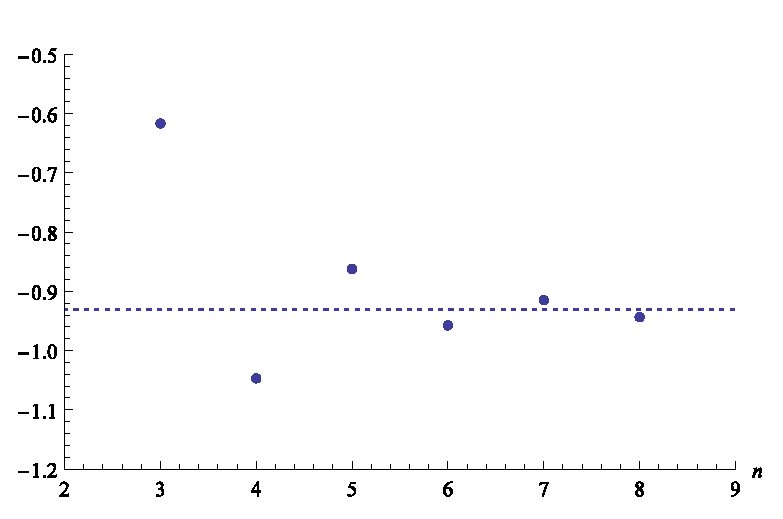
\includegraphics[scale=0.9]{../graphics/j4plot}
\caption{The dashed line shows the result from the $\bP\mu$-system for the coefficient of $S^2$ in the 1-loop energy at $J=4$, i.e. $-\frac{14 \zeta_3}{5}+\frac{48 \zeta_5}{\pi ^2}-\frac{252 \zeta_7}{\pi
   ^4}\approx-0.931$ (see \eq{gamma42weak}). The dots show the Bethe ansatz prediction \eq{gammaJ} expanded to orders $1/J^3,1/J^4,\dots,1/J^8$ (the order of expansion $n$ corresponds to the horizontal axis), and it appears to converge to the $\bP\mu$-system result.}
\label{fig:j4plot}
\end{figure}


For $J=4$ the expansion reads
\beqa
\label{gamma42weak}
	\gamma_{J=4}^{(2)}&=&g^2 \left(-\frac{14 \zeta_3}{5}+\frac{48 \zeta_5}{\pi ^2}-\frac{252 \zeta_7}{\pi
   ^4}\right)	\\ \nn
	&+&g^4 \left(-\frac{22 \pi ^2 \zeta_3}{25}+\frac{474 \zeta_5}{5}-\frac{8568 \zeta_7}{5 \pi
   ^2}+\frac{8316 \zeta_9}{\pi ^4}\right)\\ \nn
	&+&g^6 \left(\frac{32 \pi ^4 \zeta_3}{875}+\frac{3656 \pi ^2 \zeta_5}{175}-\frac{56568 \zeta_7}{25}+\frac{196128 \zeta_9}{5 \pi ^2}-\frac{185328 \zeta_{11}}{\pi ^4}\right)	\\ \nn
	&+&g^8 \left(-\frac{4 \pi ^6 \zeta_3}{175}-\frac{68 \pi ^4 \zeta_5}{75}-\frac{55312 \pi ^2 \zeta_7}{125}+\frac{1113396 \zeta_9}{25}-\frac{3763188 \zeta_{11}}{5 \pi ^2}\right.
	\\ \nn
	 && \ \ \ \ \ \  + \left.\frac{3513510 \zeta_{13}}{\pi ^4} \right)+\dots
\eeqa
Unlike for the $J=2$ and $J=3$ cases, we could not find a closed expression for the energy at any spin $S$ in literature even at one loop, however there is another way to check our result. 
One can expand the asymptotic Bethe ansatz equations at large $J$ for fixed values of $S=2,4,6,\dots$ and then extract the coefficients in the expansion which are polynomial in $S$. 
This was done in \cite{Beccaria:2012kp} (see appendix C there) where at one loop the expansion was found up to order $1/J^6$:
\beq
\label{gammaJ}
	\gamma(S,J) \simeq g^2\(\frac{S}{2\,J^{2}}-\Big(\frac{S^{2}}{4}+\frac{S}{2}\Big)\,\frac{1}{ J^{3}}
+\Big[
\frac{3 S^3}{16}+\Big(\frac{1}{8}-\frac{\pi ^2}{12}\Big) S^2+\frac{S}{2}
\Big]\,\frac{1}{ J^{4}} +\dots\)
\eeq
Now taking the part proportional to $S^2$ and substituting $J=4$ one may expect to get a numerical approximation to the 1-loop coefficient in our result \eq{gamma42weak}, i.e. $-\frac{14 \zeta_3}{5}+\frac{48 \zeta_5}{\pi ^2}-\frac{252 \zeta_7}{\pi^4}$. 
To increase the precision we extended the expansion in \eq{gammaJ} to order $1/J^8$. 
Remarkably, in this way we confirmed the 1-loop part of the $\bP\mu$ prediction \eq{gamma42weak} with about $1\%$ accuracy! 
In figure \ref{fig:j4plot} one can also see that the ABA result converges to our prediction when the order of expansion in $1/J$ is being increased.
Also, in contrast to $J=2$ and $J=3$ cases we see that negative powers of $\pi$ appear in \eq{gamma42weak}, although still all the contributions at a given loop order have the same transcendentality. 
It would be interesting to understand why this happens  from the gauge theory perspective, especially since expansion of the leading $S$ term \eq{eq:resultLO} has the same structure for all $J$,
\beq
	\gamma_{J}^{(1)}=\frac{8 \pi ^2 g^2}{J (J+1)}-\frac{32 \pi ^4 g^4}{J (J+1)^2
   (J+2)}+\frac{256 \pi ^6 g^6}{J (J+1)^3 (J+2) (J+3)}
	+\dots
\eeq
The change of structure at $J=4$ might be related to the fact that for $J\geq 4$ the ground state anomalous dimension even at one loop is expected to be an irrational number for integer $S>0$ \cite{Beccaria:2008pp,Belitsky:2008mg}, and thus cannot be written as a linear combination of harmonic sums with integer coefficients.


\subsubsection{Strong coupling expansion}
\label{sec:strong_curvature}

To obtain the strong coupling expansion of our exact results for the curvature function, we evaluated it numerically with high precision for a range of values of $g$ and then made a fit to find the expansion coefficients. 
We should note that the expansion has been carried out analytically in \cite{Beccaria:2014rca} using some clever tricks that are not obvious to justify.

For numerical study it is convenient to write our exact expressions \eq{gamma2L2}, \eq{gamma2L3}, \eq{gamma2L4} for $\gamma^{(2)}(g)$, which have the form
\beq
\label{ints}
	\gamma^{(2)}(g)=\oint {du_x}\oint {du_y} f(x,y) \partial_{u_x} \log\frac{\Gamma (i u_x-i u_y+1)}{\Gamma (1-i u_x+i u_y)}
\eeq
where the integration goes around the branch cut between $-2g$ and $2g$, in a slightly different way (we remind that we use notation $x+\frac{1}{x}=\frac{u_x}{g}$ and $y+\frac{1}{y}=\frac{u_y}{g}$). 
Namely, by changing the variables of integration to $x,y$ and integrating by parts one can write the result as
\beq
\label{ints2}
	\gamma^{(2)}(g)=\oint {dx}\oint {dy} F(x,y) \log\frac{\Gamma (i u_x-i u_y+1)}{\Gamma (i u_y-i u_x+1)}
\eeq
where $F(x,y)$ is some polynomial in the following variables: $x,\;1/x,\;y,\;1/y,\;\sh_-^x$ and $\sh_-^y$ (for $J=3$ it includes $\ch_-^x,\;\ch_-^y$ instead of the $\sh_-$ functions). 
The integral in \eq{ints2} is over the unit circle.
The advantage of this representation is that plugging in $\sh_-^x$, $\sh_-^y$ as series expansions (truncated to some large order), we see that it only remains to compute integrals of the kind
\beqa
C_{r,s}&=&\frac{1}{i}\oint\frac{dx}{2\pi}\oint\frac{dy}{2\pi}x^r y^s\log\frac{\Gamma(i u_x-iu_y+1)}{\Gamma(i u_y-iu_x+1)}
\eeqa
These are nothing but the coefficients of the BES dressing phase \cite{Beisert:2006ib, Beisert:2006ez, Vieira:2010kb, Dorey:2007xn}. 
They can be conveniently computed using the strong coupling expansion \cite{Beisert:2006ez}
\small
\beq
C_{r,s}=\sum_{n=0}^\infty\[-\frac{2^{-n-1} (-\pi )^{-n} g^{1-n} \zeta_n
   \left(1-(-1)^{r+s+4}\right) \Gamma \left(\frac{1}{2}
   (n-r+s-1)\right) \Gamma \left(\frac{1}{2}
   (n+r+s+1)\right)}{\Gamma (n-1) \Gamma \left(\frac{1}{2}
   (-n-r+s+3)\right) \Gamma \left(\frac{1}{2} (-n+r+s+5)\right)}\]
\eeq
\normalsize
However this expansion is only asymptotic and does not converge. 
For fixed $g$ the terms will start growing with $n$ when $n$ is greater than some value $N$, and we only summed the terms up to $n=N$ which gives the value of $C_{r,s}$ with very good precision for large \text{enough $g$}.
Using this approach we computed the curvature function for a range of values of $g$ (typically we took $7\leq g \leq 30$) and then fitted the result as an expansion in $1/g$. This gave us only numerical values of the expansion coefficients, but in fact we found that with very high precision the coefficients are as follows. 
For $J=2$
\beqa
\label{eq:ssj2}
\gamma^{(2)}_{J=2}&=&-\pi ^2 g^2+\frac{\pi  g}{4}+\frac{1}{8}-\frac{1}{\pi g}\(\frac{3 \zeta_3}{16}+\frac{3}{512}\)-\frac{1}{\pi^2g^2}\(\frac{9 \zeta_3}{128}+\frac{21}{512}\)\quad\quad
\\ \nn
&+&
\frac{1}{\pi^3g^3}\(\frac{3 \zeta_3}{2048}+\frac{15 \zeta_5}{512}-\frac{3957}{131072}\) + \dots\;,
\eeqa
then for $J=3$
\beqa
\label{eq:ssj3}
\gamma^{(2)}_{J=3}&=&-\frac{8 \pi ^2 g^2}{27}+\frac{2 \pi  g}{27}+\frac{1}{12}-
\frac{1}{\pi g}\(
\frac{1}{216}
+\frac{\zeta_3}{8}
\)-
\frac{1}{\pi^2g^2}\(\frac{3 \zeta_3}{64}+\frac{743}{13824}\)\quad\quad
\\ \nn
&+&
\frac{1}{\pi^3g^3}\(\frac{41 \zeta_3}{1024}+\frac{35 \zeta_5}{512}-\frac{5519}{147456}\) + \dots\;,
\eeqa
and finally for $J=4$
\beqa
\gamma^{(2)}_{J=4}&=&-\frac{\pi ^2 g^2}{8}+\frac{\pi  g}{32}+\frac{1}{16}-\frac{1}{\pi g}\(\frac{3 \zeta_3}{32}+\frac{15}{4096}\)-\frac{0.01114622551913}{g^2}\quad\quad
\\ \nn
&+&\frac{0.004697583899}{g^3}+ \dots\;.
\eeqa
To fix coefficients for the first four terms in the expansion we were guided by known analytic predictions which will be discussed below, and found that our numerical result matches these predictions with high precision. 
Then for $J=2$ and $J=3$ we extracted the numerical values obtained from the fit for the coefficients of $1/g^2$ and $1/g^3$, and plugging them into the online calculator EZFace \cite{ezface} we obtained a prediction for their exact values as combinations of $\zeta_3$ and $\zeta_5$. 
Fitting again our numerical results with these exact values fixed, we found that the precision of the fit at the previous orders in $1/g$ increased. 
This is a highly non-trivial test for the proposed exact values of $1/g^2$ and $1/g^3$ terms. 
For $J=2$ we confirmed the coefficients of these terms with absolute precision $10^{-17}$ and $10^{-15}$ at $1/g^2$ and $1/g^3$ respectively (at previous orders of the expansion the precision is even higher). 
For $J=3$ the precision was correspondingly $10^{-15}$ and $10^{-13}$.
For $J=4$ we were not able to get a stable fit for the $1/g^2$ and $1/g^3$ coefficients from EZFace, so above we gave their numerical values (with uncertainty in the last digit). 
However below we will see that based on $J=2$ and $J=3$ results one can make a prediction for these coefficients, which we again confirmed by checking that precision of the fit at the previous orders in $1/g$ increases. 
The precision of the final fit at orders $1/g^2$ and $1/g^3$ is $10^{-16}$ and $10^{-14}$ respectively.

\subsection{Update on short strings}
\label{sec:konishi_three_loops}

Having just found the curvature function we recall section \ref{sec:short_strings} where we were able to boost the folded string semi-classical energy one loop further by utilizing the knowledge of the slope function.
We also argued that knowing the curvature function would enable us to repeat the procedure and boost the result by one more loop.

The key idea was to utilize the structure of the small spin expansion \eq{eq:delta_squared_basso} of the folded string energy.
Re-expanding it at fixed global charges $S$ and $J$ we found the energy in terms of the coefficients $A_i, B_i, C_i$, etc. as seen in \eq{eq:delta_abc}.
We also found that in principle the curvature function should fix all of the $B_i$ coefficients, which we can indeed do by first expanding the curvature function at strong coupling in terms of $A$'s and $B$'s
\small
\beqa
	\label{eq:ss_abc}
	\gamma^{(2)}_{J}(g) \!\!\!\!&=&\!\!\!\! -\frac{2 \pi ^2 g^2 A_1^2 }{J^3} - \frac{\pi g A_1 A_2 }{J^3}-\frac{A_2^2+2 A_1 A_3-4 B_1 J^2}{8 J^3} - \frac{A_2 A_3+A_1 A_4-2 B_2 J^2}{16 \pi g J^3} \\
	&-&  \frac{A_3^2+2 A_2 A_4+2 A_1 A_5-4 B_3 J^2}{128 \pi^2 g^2 J^3} - \frac{A_3 A_4 + A_2 A_5 + A_1 A_6 - 2 B_4 J^2}{256 \pi^3 g^3 J^3} + \mc{O}\left(\frac{1}{g^4}\right) \nonumber
\eeqa
\normalsize
and plugging in the $A_i$ coefficients \eq{eq:bassos_as} found from the slope function.
A slight complication here is that we only have strong coupling expansions of the curvature function for $J=2,3$ and for $J=4$ we only have a numeric result. 
By comparing the $J=2,3$ expansions \eq{eq:ssj2} and \eq{eq:ssj3} to the above general form we can extract the values of the $B$'s for those two cases only.
However as discussed in section \ref{sec:short_strings} we expect all series of coefficients to have a certain power-like dependencies on $J$, namely we expect $B_1$, $B_2$ to be constant and $B_3$, $B_4$ to have the form $a J^2 + b$ with $a$ and $b$ constant.
Having just found two data points for $J=2,3$ we immediately find $a$ and $b$ and thus deduce that
\beqa
 \begin{array}{rcrlrlrcl}
B_1 &=& &3/2, &B_2& &=& &-3\,\zeta_3+\frac{3}{8}, \nn \\
B_3 &=& &-\frac{J^2}{2}-\frac{9 \, \zeta_3}{2}+\frac{5}{16}, &B_{4}& &=& &\frac{3}{16} J^2 (16 \, \zeta_3+20 \, \zeta_5-9)-\frac{15 \, \zeta_5}{2}-\frac{93 \, \zeta_3}{8}-\frac{3}{16}.
\end{array}
\eeqa
Having fixed all the unknowns we can now write the strong coupling expansion of the curvature function for arbitrary values of $J$ as
\small
\beqa
 \gamma^{(2)}_{J}(g) &=& -\frac{8 \pi ^2 g^2}{J^3}+\frac{2 \pi  g}{J^3}+\frac{1}{4 J}+\frac{1-J^2 (24 \, \zeta_3 +1)}{64 \pi  g J^3} - \frac{8 J^4+J^2 (72 \, \zeta_3 +11)-4}{512 g^2 \left(\pi ^2 J^3\right)}  \nonumber \\
  &+& \frac{3 \left(8 J^4 (16 \, \zeta_3 +20 \, \zeta_5-7)-16 J^2 (31 \, \zeta_3 +20 \, \zeta_5+7)+25\right)}{16384 \pi ^3 g^3 J^3} + \mc{O}\left(\frac{1}{g^4}\right).\qquad\qquad
\eeqa
\normalsize
Expanding $\gamma^{(2)}_{J=4}$ defined in \eq{gamma2L4} at strong coupling numerically we were able to confirm the above result with high precision.


\begin{table}[t]
\begin{tabular}{|l||rl|l|l||l|l|l|}
  \hline
  $(S,J)$ & \multicolumn{2}{|l|}{$\lambda^{-5/4}$ prediction} & $\lambda^{-5/4}$ fit & error & fit order\\
  \hline
  $(2,2)$ & $\frac{15 \, \zeta_5}{2} + 6 \, \zeta_3-\frac{1}{2}$&$= 14.48929958$ & $14.12099034$ & $2.61\%$ & 6\\
  $(2,3)$ & $\frac{15 \, \zeta_5}{2} + \frac{63 \, \zeta_3}{8} - \frac{1131}{512}$&$= 15.03417190$ & 14.88260078 & $1.02\%$ & 5 \\
  $(2,4)$ & $\frac{21 \, \zeta_3}{2} + \frac{15 \, \zeta_5}{2} - \frac{25}{8}$&$= 17.27355565$ & $16.46106336$ & $4.94\%$ & 7\\
  \hline
\end{tabular}
\caption{Comparisons of strong coupling expansion coefficients for $\lambda^{-5/4}$ obtained from fits to TBA data versus our predictions for various operators. The fit order is the order of polynomials used for the rational fit function (see \cite{Gromov:2011bz} for details).}
\label{tab:coefficients}
\end{table}

Now that we know the strong coupling expansion of the curvature function and thus all the coefficients $B_i$, we can do the same trick and find the three loop strong coupling scaling dimension coefficient $\Delta^{(3)}$, which now depends on $A_{1;2;3;4}$, $B_{1,2,3}$, $C_{1,2}$, $D_1$. We find it to be
\beqa
	\Delta^{(3)} &=& \frac{187\,S^6 + 2\,(624\,\zeta_3 + 480\,\zeta_5-193)\,S^5 +\left(-146\,J^2 - 4\,(336\,\zeta_3-41)\right)S^4 }{512 \sqrt{2}\,S^{5/2}} + \nonumber \\
	&+& \frac{\left(32\,(6\,\zeta_3+7)\,J^2-88\right)S^3 + \left(-28\,J^4 + 40\,J^2\right) S^2 - 24\,J^4 S + 8\,J^6}{512 \sqrt{2}\,S^{5/2}},
\eeqa
for $S=2$ it simplifies to
\beq
	\Delta^{(3)}_{S=2} = \frac{1}{512} \left(J^6-20 J^4+48 J^2 (4 \zeta_3 - 1)+192 (12 \, \zeta_3+20 \, \zeta_5+1)\right)
\eeq
and finally for the Konishi operator, which has $S=2$ and $J=2$ we get
%\footnote{The $\zeta_3$ and $\zeta_5$ terms are coming from semi-classics and were already known before \cite{Beccaria:2012xm} and match our result.}
 \beq
  \Delta^{(3)}_{S=2,J=2} = \frac{15 \, \zeta_5}{2} + 6 \, \zeta_3-\frac{1}{2}.
 \eeq
In order to compare our predictions with numeric data available from explicit Y-system calculations \cite{Frolov:2010wt}, we employed Pad\'{e} type fits as explained in \cite{Gromov:2011bz}. 
The fit results are shown in table \ref{tab:coefficients}, we see that our predictions are within $5\%$ error bounds, which is a rather good agreement. 
However we must be honest that for the $J=3$ and especially $J=4$ states we did not have as many data points as for the $J=2$ state and the fit is somewhat shaky.


\subsection{Cusped Wilson line}
\label{sec:wilson_line}

\begin{figure}[t]
\centering
\begin{tikzpicture}
	
	%\draw[help lines] (0,0) grid (15,5);
	
	\draw[->,dotted,very thick] (1,1) -- (2,1);
	\draw[->,very thick] (2,1) -- (7,1) -- (12,4);
	\draw[dotted,very thick] (12,4) -- (12.5,4.3);
	\draw[dashed,very thick] (7,1) -- (13,1);
	
	\node[draw,circle,fill=white] at (7,1) {$Z^L$};
	
	\draw[] (8.5,1) to [out=90,in=-30] (8.1,1.66);

	\node at (4,1.5) {\Large $\vec{n}$};
	\node at (10,3.5) {\Large $\vec{n_\theta}$};
	\node at (9,1.6) {\Large $\phi$};
	
\end{tikzpicture}
\caption{The cusped Wilson line with an operator insertion.}
\label{fig:wilson_line}
\end{figure}

In this section we will consider an observable illustrated in figure \ref{fig:wilson_line}, it consists of two rays of a supersymmetric Wilson line forming a cusp with the angle $\phi$ and an operator $Z^L$ inserted at the cusp, where $Z$ is a scalar of ${\cal N}=4$ super Yang-Mills. 
To completely define a supersymmetric Wilson line we should also specify the coupling to scalars, which is parametrized by a six-dimensional unit vector $\vec n(t)$ at each point of the line, where $t$ is a parameter on the line. 
In our case $\vec n(t)$ is constant and equal $\vec n$ on one ray and $\vec n_\theta$ on another ray, so that $\vec n\cdot \vec n_\theta=\cos\theta$. 
Because of R-symmetry the observable depends on $\vec n,\vec n_\theta$ only through $\theta$.
Explicitly the observable is defined as
\beq
\label{WilsL}
	W_L={\rm P}\exp\!\int\limits_{-\infty}^0\! dt\(i  A\cdot\dot{x}_q+\vec\Phi\cdot\vec n\,|\dot x_q|\)\times Z^L\times {\rm P}\exp\!\int\limits_0^\infty\!dt\(i A\cdot\dot x_{\bar q}+\vec\Phi\cdot\vec n_\theta\,|\dot x_{\bar q}|\).
\eeq
Due to the cusp the expectation value of such an observable diverges as
\beq
\left\langle W_L\right\rangle \sim \(\frac{\Lambda_{IR}}{\Lambda_{UV}}\)^{\Gamma_L(\lambda)},
\eeq
where $\Lambda_{IR}$ and $\Lambda_{UV}$ are the infra-red and ultraviolet cut-offs respectively \cite{Polyakov:1980ca,Correa:2012at}. 
The quantity $\Gamma_{L}$, which we will call the cusp anomalous dimension, will be the main object of our study in this section.
The AdS/CFT duality allows one to relate the observable in ${\cal N}=4$ SYM described above to an open string in $\adsfive$ which ends on a cusped line on the boundary of AdS. In particular, in the classical scaling limit when $L$ and $\lambda$ are both taken to infinity with $L/\sqrt{\lambda}$ fixed, we can match $\Gamma_{L}$ with the energy of the classical string \cite{Correa:2012hh, Gromov:2012eu}.

Wilson lines are non-local observables in the sense that they are parametrized by a line in spacetime instead of just a point.
Technically this renders the whole machinery of spin chains and spectral curves unsuitable for studying these observables as we assumed to be working with local operators. 
Remarkably it turns out that cusped Wilson lines are very similar to local single trace operators.
They key idea is to consider the insertion of the local operator $Z^L$ at the cusp as an open spin chain with the Wilson lines imposing certain boundary conditions for the magnons inside the chain \cite{Drukker:2012de}.
One can then write down Bethe ansatz equations with a modified $S$-matrix incorporating the boundary conditions and find the cusp anomalous dimension at weak coupling.
Remarkably a set of thermodynamic Bethe ansatz equations have also been found for this observable, which also go by the name of twisted boundary thermodynamic Bethe ansatz equations (abbreviated by TBTBA, BTBA or TBA) \cite{Correa:2012hh}.
In the small $\phi$ and $\theta=0$ limit the equations can be dramatically simplified and cast in a FiNLIE form, which even admits an analytic solution \cite{Gromov:2012eu}, later generalized \cite{Gromov:2013qga} to the case of arbitrary but close to each other angles $\theta^2-\phi^2\rightarrow 0$. 
In this general case the cusp anomalous dimension was found to be
\beq
\label{eq:mainresultIntro}
\Gamma_L(\lambda)=\frac{\phi-\theta}{4}\partial_\theta\log\frac{\det{\cal M}_{2L+1}}{\det{\cal M}_{2L-1}}+{\cal O}((\phi-\theta)^2),
\eeq
where ${\cal M}_N$ is an $(N+1)\times (N+1)$ sized matrix defined as
\begin{align}
\label{eq:M}
&\({\cal M}_N\)_{ij} =I^\theta_{i-j+1},\\
&I_n^\theta =i^{n+1}I_n\(\frac{\sqrt{\lambda}}{\sin\beta}\)\sin{n\beta}, \;\;\;\; \mathrm{with} \;\; \sin{\beta}=\frac{1}{\sqrt{1-\theta^2/\pi^2}},
\nonumber
\end{align}
and $I_n(x)$ are modified Bessel functions of the first kind. 
When $\theta^2-\phi^2=0$ the observable $W_L$ becomes BPS and the cusp anomalous dimension vanishes \cite{Drukker:2006xg}. 

\subsubsection{$\pmu$-system solution}

Since a Y-system of equations can be written down for the cusped Wilson line it is then hardly a surprise that it can also be studied using the quantum spectral curve construction, as was shown in \cite{Gromov:2013pga}. 
We will briefly review the solution for the small $\phi$ case.
The $\pmu$-system has the same general form as given in \eq{Pt}, \eq{muPPt-eq} and what distinguishes this case from the $\alg{sl}{2}$ sector are the asymptotics.
They can be read off from the Y-system solution and shown to be \cite{Gromov:2013pga}
\beq
	\label{eq:cusp_pmu_asymptotics}
	\bP_a \simeq \( A_1 u^{-L+1/2}, A_2 u^{-L-1/2}, A_3 u^{+L+3/2}, A_4 u^{+L+1/2} \).
\eeq
The algebraic constraints on $A_i$'s suggest that at $\phi=0$ one has $A_2 A_3 \simeq A_4 A_1 \to 0$, which in turn implies that $\bP_a = 0$ to leading order in $\phi$.
This can be seen by analogy with the $\alg{sl}{2}$ sector constraints \eq{AA1} - \eq{AA2}, which although not technically valid for this case still capture the correct behaviour at small $\phi$ by setting the spin $S=0$ and $\Delta = L +\ord{\phi^2}$.
Since to leading order $\bP$'s are small we find from the $\pmu$-system that $\tilde{\mu}_{ab} = \mu_{ab}$ and thus it has no cuts and is just a periodic function as follows from \eq{muper}.
Another feature of the Y-system in this case is that due to the boundary dressing phase the product $Y_{11} Y_{22}$ contains poles at $u= i n/2$ for integer $n \neq 0$ \cite{Correa:2012hh}, thus from \eq{eq:y_asymp} we deduce that 
\beq
	\mu_{12} = C \sinh (2 \pi u),
\eeq
where we also used the fact that $\mu_{12}$ has to be odd for vacuum states, the origin of which lies in the Y-system equations.
Such parity requirements also apply to other $\mu_{ab}$'s which we assume to be constant, together with the constraints \eq{constraint} - \eq{constraint2} thus fixing them to be
\beq
	\mu_{13} = \mu_{24} = \mu_{34} = 0, \;\; \mu_{14} = -1.
\eeq
The $\pmu$-system finally reduces to the following set of equations
\beqa
	\tilde{\bP}_1 - \bP_1 &=& -C \sinh \( 2\pi u \) \bP_3, \label{eq:cusp_p1} \\
	\tilde{\bP}_2 + \bP_2 &=& -C \sinh \( 2\pi u \) \bP_4, \label{eq:cusp_p2} \\
	\tilde{\bP}_3 + \bP_3 &=& 0, \label{eq:cusp_p3} \\ 
	\tilde{\bP}_4 - \bP_4 &=& 0. \label{eq:cusp_p4} 
\eeqa
Let us consider the $L=0$ case for simplicity.
First thing we notice is that \eq{eq:y_asymp} should not have a pole at $u=0$, thus we have to set $\bP_1 \bP_2 = 0$ at $u=0$, which we do by introducing factors of $\sqrt{u}$ in order to comply with the asymptotics \eq{eq:cusp_pmu_asymptotics}.
From \eq{eq:cusp_p4} we see that
\beq
	\bP_4 = A_4 \sqrt{u},
\eeq	
as it does not change sign when crossing the cut, meanwhile from \eq{eq:cusp_p3} we get
\beq
	\bP_3 = A_3 \sqrt{u} \sqrt{u^2 - 4g^2},
\eeq
as it does change sign when crossing the cut $u \in [-2g, 2g]$.
From \eq{eq:cusp_p2} we can find $\bP_2$ which is given by a Hilbert transform of $\sinh(2\pi u)$,
\beq
	\frac{-\bP_2}{C A_4 \sqrt{u}} = \oint_{-2g}^{2g} \frac{\sqrt{u^2-4g^2}}{\sqrt{v^2-4g^2}} \frac{\sinh(2\pi v)}{4 \pi i (v-u)} = \sum_{n=1}^\infty \frac{I_{2n-1}(4\pi g)}{x^{2n-1}},
\eeq
furthermore we find that $A_2 = -g\, C A_4\, I_1 \( 4 \pi g \)$.
Finally the solution for $\bP_1$ can be easily verified to be
\beq
	\bP_1 = -\frac{A_3}{A_4} \sqrt{u^2 - 4g^2} \, \bP_2 + \( A_1 + \frac{A_3 A_2}{A_4} \) \sqrt{u}.
\eeq
Now we introduce the angle $\phi$ and energy $\Delta$ by comparing to the Y-system asymptotics when $u \to \infty$,
\beqa
	Y_{11} + 1 &\simeq& -\frac{\phi^2}{2} \\
	Y_{11} Y_{22} - 1 &\simeq& \frac{2 i \Delta}{u},
\eeqa
where the last equation only differs by the factor of 2 from the $\alg{sl}{2}$ case \eq{eq:y1122_sl2_asymptotics}.
First we notice that $A_1 A_4 = A_2 A_3$, since otherwise $Y_{11} Y_{22} - 1$ would grow linearly, then we find $A_1 A_4 = i \phi^2$, thus fixing the energy to be
\beq
	\Delta = -\phi^2 g^2 \(1 - \frac{I_3(4\pi g)}{I_1(4\pi g)} \),
\eeq
which exactly reproduces the TBA result \eq{eq:mainresultIntro} for $L=0$ and $\theta=0$.
The general case can also be reproduced with just a bit more effort. 
We should also note that this result was also found in a completely different manner by utilizing localization techniques \cite{Correa:2012at,Fiol:2012sg}, thus confirming the validity of the $\pmu$-system approach.

\subsubsection{Matrix model formulation}
\label{sec:wilson_classical}

An obvious complication in the formulation of the result \eq{eq:mainresultIntro} is that it contains determinants of $(2L+1)\times (2L+1)$ sized matrices, which is very problematic if one wants to take the large $L$ limit. 
It becomes considerably easier once we realize that the cusp anomalous dimension can be expressed in terms of an expectation value of some operator in a matrix model. 
%In this section we will show how to use this approach to find the large $N$ expansion of the determinant of ${\cal M}_N$ defined in \eq{eq:M}.
One can check that the quantities $I^\theta_n$ defined in the previous section can be rewritten in the following integral representation
\begin{equation}
	I_n^\theta = \frac{1}{2\pi i} \oint \frac{dx}{x^{n+1}} \sinh(2\pi g \, (x + 1/x)) \, e^{2 g \theta (x - 1/x)},
\end{equation}
where the integration contour is the unit circle and $g=\frac{\sqrt\lambda}{4\pi}$. 
This makes it possible to write the determinant of ${\cal M}_{N}$ as
\beq
\det \M_{N}=
\oint\prod_{i=1}^{N+1}\frac{dx_i}{2\pi i} e^{2 g \, \theta \left(x_i-\frac{1}{x_i}\right)} \sinh \left(2 \pi g \left( x_i + \frac{1}{x_i} \right) \right) \times \det X,
\eeq
where
\beq
\det X = \left|
\bea{lllll}
x_1^{-2}&x_1^{-1}&\dots&x_1^{N-1}&x_1^{N-2}\\
x_2^{-3}&x_2^{-2}&\dots&x_2^{N}&x_2^{N-1}\\
\vdots&\vdots& \ddots & \vdots& \vdots\\
x_{N}^{-N-1}&x_{N}^{-N}&\dots&x_{N}^{-2}&x_{N}^{-1}\\
x_{N+1}^{-N-2}&x_{N+1}^{-N-1}&\dots&x_{N+1}^{-3}&x_{N+1}^{-2}
\eea
\right| = \frac{\prod_{i<j}^{N+1} (x_i - x_j)}{\prod_{i=1}^{N+1} x_i^{i+1}},
\eeq
and we recognize the numerator as the Vandermonde determinant $\Delta(x_i)$. 
We can further simplify the final result by anti-symmetrizing the denominator, which we can do because everything else in the integrand is anti-symmetric and the integration measure is symmetric w.r.t $x_i$, thus under the integral we can replace $\det X$ by
\beq
	\det X' = \frac{\Delta^2(x_i)}{(N+1)!} \, \prod_{i=1}^{N+1} \frac{1}{x_i^{N+2}}.
\eeq
Thus finally we get the following expression
\begin{equation}
  \det \M_{N} = \frac{1}{(2 \pi i)^{N+1}} \oint \prod_{i=1}^{N+1} \frac{d x_i}{x_i^{N+2}} \, \frac{\Delta^2(x_i)}{(N+1)!}  \, \sinh(2\pi g \, (x_i + 1/x_i)) \, e^{2 g \theta (x_i - 1/x_i)},
  \label{eq:Mintegral}
\end{equation}
which indeed has the structure of a partition function of some matrix model.
%\footnote{Namely, it is equal to the partition function of a two-matrix model. We thank I.Kostov for discussions related to this question.}. 
It now becomes a matter of simple algebra to convince oneself that the cusp anomalous dimension \eq{eq:mainresultIntro} can be written in terms of expectation values in this matrix model, namely
\beq
	\Gamma_L(g) = g \, \frac{\phi-\theta}{2} \left[ \,\, \left< \sum_{i=1}^{2L+1} \( x_i - \frac{1}{x_i}\)  \right>_{2L+1} - \,\,\, \left<  \sum_{i=1}^{2L-1} \(x_i - \frac{1}{x_i}\) \right>_{2L-1} \right],
\eeq
where $\left< \dots \right>_{N}$ denotes the normalized expectation value in the matrix model of size $N$ with the partition function defined in (\ref{eq:Mintegral}). 
Note that this formula is exact and we have not yet taken any limits.

\subsubsection{Classical limit}

As already mentioned before, when $L$ and $\lambda$ are both taken to infinity with $L/\sqrt{\lambda}$ fixed the cusp anomalous dimension $\Gamma_L(\lambda)$ can be matched to the energy of a classical open string solution.
In this subsection we will take this limit of the exact result \eq{eq:mainresultIntro} and in the next subsection we will do the matching to the string result.
Alternatively since we already saw that the problem can be solved with the quantum algebraic curve construction, one would expect to be able to start from the string solution and apply the classical spectral curve techniques as discussed in section \ref{sec:spectral_curve}. 
Technically the algebraic curve is defined for closed string solutions, however there is evidence that the construction can be easily generalized for open strings by trivially modifying the definition of the monodromy \eq{eq:monodromy} \cite{Janik:2012ws}.
This evidence is strongly supported by our derivation which looks remarkably similar to the $\alg{sl}{2}$ classical spectral curve construction.
Because of this we will loosely refer to our result as the algebraic curve.

We will be utilizing the matrix model reformulation of the cusp anomalous dimension as discussed in the previous subsection. 
As usual in matrix models, when the size of matrices becomes large, the partition function is dominated by the solution of the saddle point equations. 
In the leading order it is just equal to the value of the integrand at the saddle point. 
%We start with this approximation, commenting shortly on the first correction in section \ref{sec:The1loop}. 
We start by recasting the partition function \eq{eq:Mintegral} into the form\footnote{we take $N=2L$.}
\beq
	\det \M_{2L} = \frac{1}{(2 \pi i)^{2L+1}} \frac{1}{(2L+1)!} \, \oint \prod_{i=1}^{2L+1} d x_i \, e^{-S(x_1, x_2, \dots, x_{2L+1})},
\eeq
where the action is given by
\begin{eqnarray}
	S &=& \sum_{i=1}^{2L+1} \[ 2 g \theta  \( x_i - \frac{1}{x_i} \)  - \(2L + 2\) \log x_i \] + 2 \sum_{i<j}^{2L+1} \log(x_i - x_j) + \\ \nonumber
	       &+& \sum_{i=1}^{2L+1} \log \sinh \( 2 \pi g \( x_i + \frac{1}{x_i} \) \).
\end{eqnarray}
The saddle point equations $\partial S / \partial x_j = 0$ now read\footnote{Technically the $x_j^{-1}$ term has a coefficient of $L+1$, but since we are taking $L \rightarrow \infty$ we chose to neglect it for simplicity.}
\begin{equation}
	g \theta \left( 1 + \frac{1}{x_j^2} \right) - \frac{L}{x_j} + \sum_{i \neq j}^{2L+1} \frac{1}{x_j - x_i} + \pi g \left( 1- \frac{1}{x_j^2} \right) \coth \left( 2 \pi g \left( x_j + \frac{1}{x_j} \right) \right) = 0.
\end{equation}
We can further simplify them by noting that a large coupling constant $g$ appears inside the cotangent and since the roots $x_i$ are expected to be of order 1, with exponential precision it is possible to replace
\begin{equation}
	\coth \left( 2 \pi g \left( x_j + \frac{1}{x_j} \right) \right) \approx \mathrm{sgn}(\mathrm{Re}(x_j)).
\end{equation}
Finally we bring the equations to a more canonical and convenient form and get the following result,
\begin{equation}
	-\theta \, \frac{x_j^2 + 1}{x^2_j - 1} + \frac{L}{g} \frac{x_j}{x_j^2 - 1} - \frac{1}{g} \frac{x_j^2}{x_j^2 - 1} \sum_{i \neq j}^{2L+1} \frac{1}{x_j - x_i} = \pi \, \mathrm{sgn}(\mathrm{Re}(x_j)).
	\label{eq:saddlepoint}
\end{equation}
An alternative way of finding these values $x_i$ is to consider the following quantity $P_L(x)$, which played an important role in \cite{Gromov:2012eu},
\beq
P_L(x)=\frac{1}{\det {\cal M}_{2L}}\left|\begin{matrix}
I_1^{\theta}& I_0^{\theta}& \cdots & I_{2-2L}^{\theta}  &I_{1-2L}^{\theta}\\
I_2^{\theta}& I_1^{\theta}& \cdots & I_{3-2L}^{\theta} &I_{2-2L}^{\theta}\\
\vdots      &  \vdots     &\ddots & \vdots            &\vdots           \\
I_{2L}^{\theta}& I_{2L-1}^{\theta}& \cdots & I_{1}^{\theta}  &I_{0}^{\theta}\\
x^{-L}& x^{1-L}& \cdots & x^{L-1} &x^{L}\\
\end{matrix}\right|.
\label{eq:PLrepr}
\eeq
The numerator is the same as $\det \M_{2L}$ except in the last line $x_{2L+1}$ is replaced by $x$ which is not integrated over. 
In the classical limit all integrals are saturated by their saddle point values, i.e. one can remove the integrals by simply replacing $x_i \rightarrow x_i^{cl}$. 
If we replace $x$ with any saddle point value $x_i^{cl}$ the determinant will contain two identical rows and will automatically become zero, thus the zeros of $P_L(x)$ are the saddle point values. 
On the complex plane they are distributed on two arcs as shown in figure \ref{fig:roots}. 
As expected, for the case $\theta=0$ we recover two symmetric arcs on the unit circle \cite{Gromov:2012eu}.
\begin{figure}[t]
	\centering
		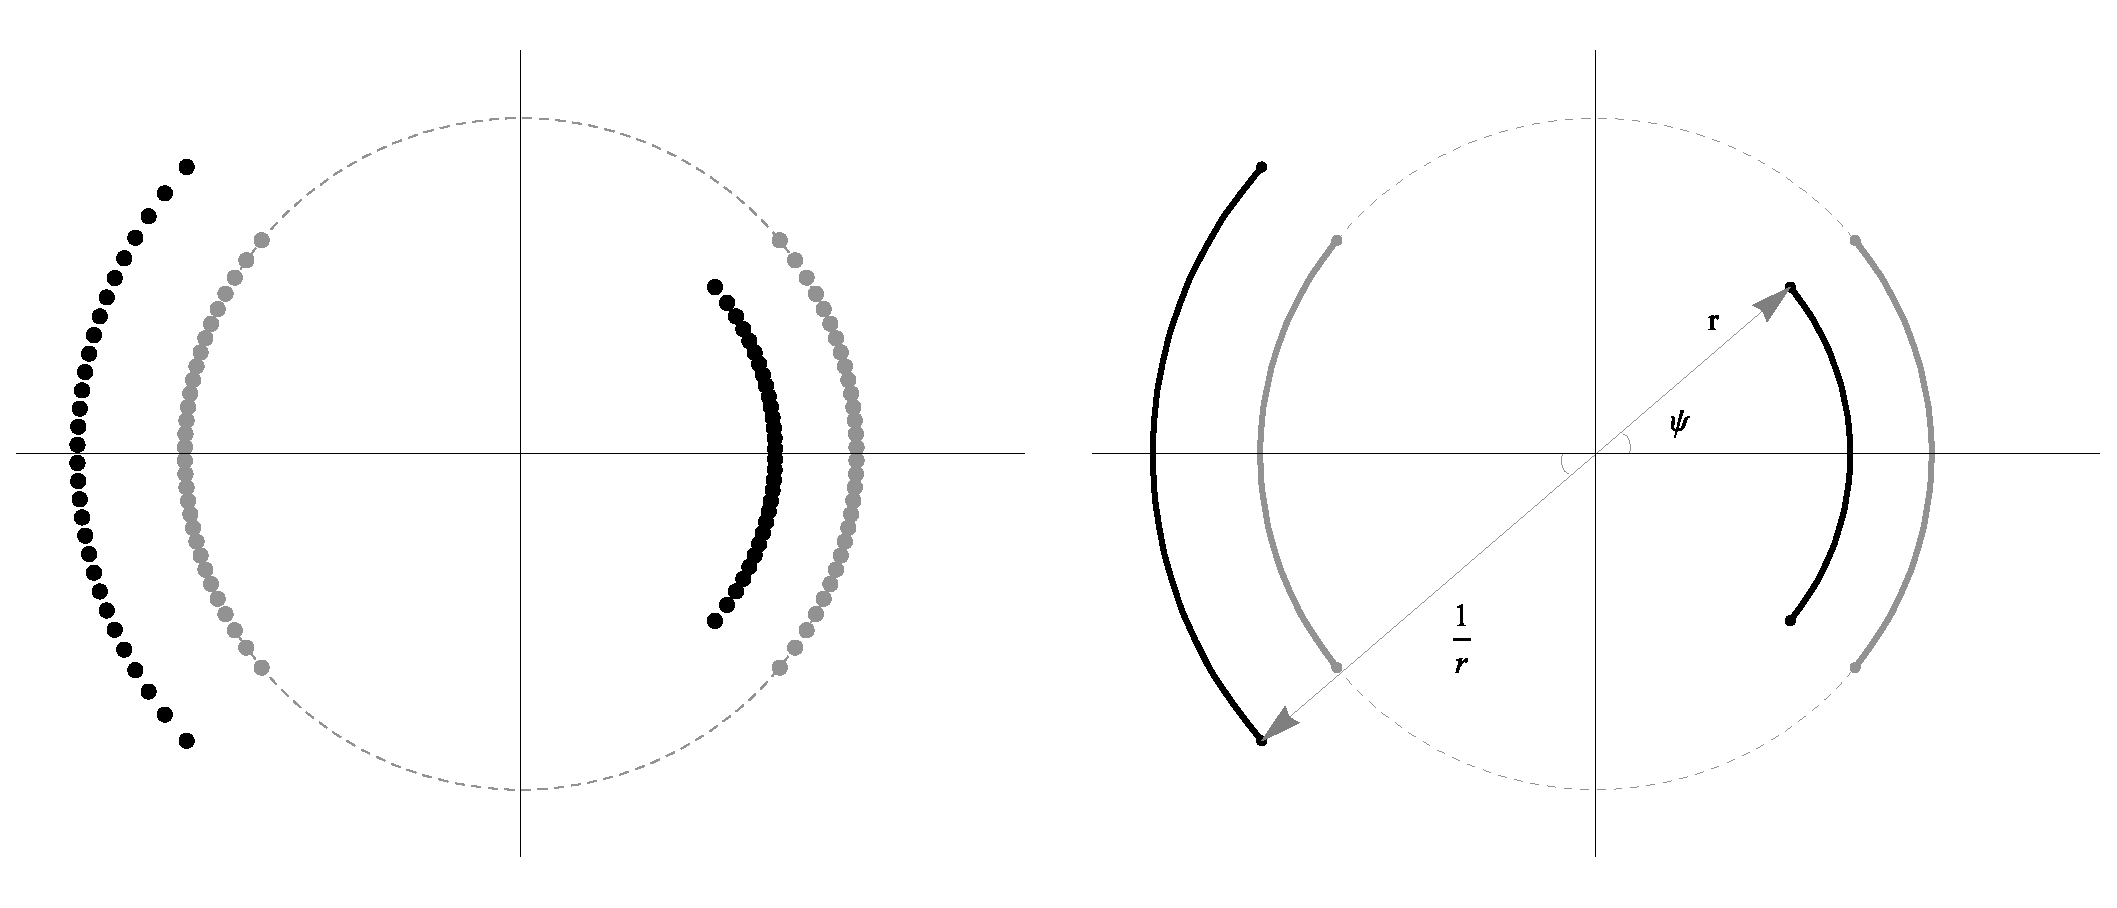
\includegraphics[width=0.95\textwidth]{../graphics/roots_cuts}
	\caption{Distribution of roots on the complex plane for $\theta=0$ (gray) and $\theta=1$ (black) on the left and the condensation of the roots to corresponding smooth cuts on the right with the algebraic curve parameters $r$ and $\psi$ identified. The dashed circle is the unit circle.}
	\label{fig:roots}
\end{figure}
Now, following \cite{Gromov:2012eu,Beisert:2005bm,Gromov:2007aq}, we introduce the quasi-momentum $p(x)$ as
\begin{equation}
	p(x) = -\theta \, \frac{x^2 + 1}{x^2 - 1} + \frac{L}{g} \frac{x}{x^2 - 1} - \frac{2L}{g} \frac{x^2}{x^2 - 1} \, G_L(x),
	\label{eq:quantum_quasimomentum}
\end{equation}
where the resolvent $G_L(x)$ is
\begin{equation}
	G_L(x) = \frac{1}{2L} \sum_{k=1}^{2L+1} \frac{1}{x-x_k}.
	\label{eq:resolvent}
\end{equation}
The motivation for introducing $p(x)$ is that  the saddle point equations (\ref{eq:saddlepoint}) expressed through $p(x)$ take a very simple form
\begin{equation}
	\frac{1}{2} \left( p(x_i + i \epsilon) + p(x_i - i \epsilon) \right) = \pi \, \mathrm{sgn}(\mathrm{Re}(x_i)).
	\label{eq:pepsilon}
\end{equation}
In the classical limit the poles in the quasi-momentum condense and form two cuts. The shifts $\pm i\epsilon$ in the equation above refer to taking the argument of the quasi-momentum to one or the other side of the cut.

In the classical limit the poles of $p(x)$, which we denote as $x_i$, are governed by the saddle-point equation and condense on two cuts in the complex plane, as shown in figure \ref{fig:roots}.
The saddle-point equation \eq{eq:saddlepoint} has a symmetry $x\rightarrow -1/x$, so does the set of poles $x_i$. 
For the quasi-momentum (\ref{eq:quantum_quasimomentum}) this symmetry manifests as the identity $p(x) = -p(-1/x)$. 
Thus we conclude that the two cuts are related by an $x\rightarrow -1/x$ transformation. 
This and the invariance of the saddle-point equation under complex conjugation implies that the four branch points can be parametrized as $\{r\,e^{i\psi},r \, e^{-i\psi},-1/r \, e^{i\psi},-1/r \, e^{-i\psi}\}$. 
Note that in the case $\theta=0$ the symmetry is enhanced to $p(x)=-p(-x)$ and $p(1/x) = p(x)$, which is not true for arbitrary $\theta$.

The crucial point to notice is that while $p(x)$ satisfies the equation \eq{eq:pepsilon} which has different constants on the right hand side for the two different cuts, the corresponding equation for $p'(x)$ has a zero on the right hand side for both cuts, thus we expect $p'(x)$ to have a simpler form than $p(x)$. 
Our strategy is to write down an ansatz for the derivative $p'(x)$ using the symmetries and analytical properties of $p(x)$ and then integrate it. 
The form of the expression we get is analogous to the curve constructed in \cite{Kazakov:2004qf}, which also helps us to construct the ansatz.

First, $p(x)$ has four branch points and according to \eq{eq:pepsilon} its derivative changes sign on each cut, hence all the cuts are of square-root type. One can write $p'(x)\propto 1/y(x)$, where
 \beq
 	y(x) = \sqrt{x-r e^{i \psi}}\sqrt{x-r e^{-i \psi}}\sqrt{x + \frac{1}{r} e^{i \psi}}\sqrt{x + \frac{1}{r} e^{-i \psi}}.
 \label{eq:y}
 \eeq
Second, since the algebraic curve is obtained from \eq{eq:quantum_quasimomentum} in the classical limit, $p(x)$ should have simple poles at $x=\pm 1$. 
Finally, from \eq{eq:quantum_quasimomentum}  we can get the behaviour at infinity:
\beq
	p'(x) \approx \frac{L}{g} \frac{1}{x^2} + \mathcal{O}\(\frac{1}{x^3}\).
\eeq
By using the knowledge about these singularities and asymptotics we can fix $p(x)$ completely. 
Based on what we know up to now we write down our ansatz for the derivative
\beq
	p'(x) = \frac{A_1 x^4 + A_2 x^3 + A_3 x^2 + A_4 x + A_5}{(x^2 - 1)^2 \, \sqrt{x-r e^{i \psi}}\sqrt{x-r e^{-i \psi}}\sqrt{x + \frac{1}{r} e^{i \psi}}\sqrt{x + \frac{1}{r} e^{-i \psi}}}.
\eeq
The polynomial in the numerator is of order four in order to maintain the correct asymptotics, and below we fix its coefficients using the properties of the quasi-momentum. 
Of course, comparing with the asymptotic one can immediately see that $A_1 = L/g$, however our objective is to express $p(x)$ solely in terms of $r$ and $\psi$, which parametrize the algebraic curve.
The $x\rightarrow-1/x$ symmetry for the derivative implies that $A_1 = A_5$ and $A_2 = -A_4$. 
Next, simple poles at $x=\pm 1$ in $p(x)$ require zero residues of $p'(x)$ at $x=\pm1$, which fixes $A_2$ to be
\beq
	A_2 =- \frac{(2A_1 + A_3) \, r \, (r^2 - 1) \cos \psi}{r^4 - 2 \, r^2 \, \cos 2\psi + 1}.
\eeq
We fix the two remaining unknowns $A_1$ and $A_3$ after integrating the $p'(x)$. 
We don't write the intermediate results of the integration as the expressions are enormous without any apparent structure.
Looking back at \eq{eq:pepsilon} we see that at the branchpoints
\beq
	p(x_{bp}) =\pm \pi.
\eeq
We use this condition to fix $A_1$ and we get
\beq
	A_1 = \frac{A_3}{2}\frac{K_1-E_1}{E_1+K_1-2\,a^2 \, K_1\cos^2(\psi)},
\eeq
where
\beq
E_1=\mathbb{E}\(a^2\sin^2(\psi)\),\;K_1=\mathbb{K}\(a^2\sin^2(\psi)\),\;a = \frac{2r}{r^2+1}.
\label{eq:E1K1}
\eeq
Finally we can use the $x \rightarrow -1/x$ symmetry on the quasi-momentum itself, as before we only used it on the derivative. Imposing the symmetry yields
\beq
	A_3 = \frac{8}{a}\(E_1+K_1-2\,a^2\,\cos^2(\psi)K_1\).
\eeq
As expected, after plugging these coefficients into $p(x)$ the whole expression simplifies enormously and we are left with our main result
\begin{align}
	\label{eq:pmainresult}
	p(x) &= \pi - 4\,i\,  E_1\, \mathbb{F}_1(x) + 4\,i\,  K_1\, \mathbb{F}_2(x) - a \left( \frac{x+ r e^{-i\psi}}{x+\frac{1}{r} e^{i\psi}} \right) \left(\frac{2/r\,e^{i \psi}}{x^2 - 1} \right) y(x)\,K_1,
\end{align}
where
\begin{equation}
	\mathbb{F}_1(x) = \mathbb{F}\left( \left. \sin^{-1} \sqrt{ \left( \frac{x -r e^{-i\psi}}{x+ \frac{1}{r} e^{i\psi}} \right) \left( \frac{ e^{ i \psi}}{ia\,r\sin\psi} \right)} \; \right| a^2 \sin^2(\psi) \right),
\end{equation}
\begin{equation}
	\mathbb{F}_2(x) = \mathbb{E}\left( \left. \sin^{-1} \sqrt{ \left( \frac{x -r e^{-i\psi}}{x+ \frac{1}{r} e^{i\psi}} \right) \left( \frac{ e^{ i \psi}}{ia\,r\sin\psi} \right) } \; \right| a^2 \sin^2(\psi) \right).
\end{equation}
We verified this result numerically by comparing it to the extrapolation of the discrete quasi-momentum \eq{eq:quantum_quasimomentum} at large $L$ and got an agreement up to thirty digits. 
We also compared this expression at $\theta = 0$ with the quasi-momentum obtained in \cite{Gromov:2012eu} and the expressions agree perfectly.
The resulting quasi-momentum is parametrized in terms of the branchpoints, i.e. the parameters are the radius $r$ and angle $\psi$. 
They are determined in terms of $L/g$ and $\theta$, which are parameters of the matrix model. 
We already mentioned that $L/g$ is simply the constant $A_1$, which we found to be
\beq
	\frac{L}{g} = 4\,\frac{K_1-E_1}{a} ,
	\label{eq:Lgfixed}
\eeq
and looking back at \eq{eq:quantum_quasimomentum} we see that $\theta = p(0) = -p(\infty)$, hence
\beqa
	\theta &=& -\pi + \frac{2a}{r}\,e^{i\psi}K_1 \nonumber \\
	       &-& \left. 4 \, i \, K_1\,\mathbb{E}\left(\sin ^{-1}\sqrt{\frac{  e^{i\psi}}{ia\,r\sin\psi}} \,\right|\, a^2 \sin ^2(\psi )\right)\nonumber \\
           &+& \left. 4 \, i \, E_1\, \mathbb{F}\left(\sin ^{-1}\sqrt{\frac{  e^{i\psi}}{ia\,r\sin\psi}}\,\right|\, a^2 \sin ^2(\psi )\right).
           \label{eq:thetafixed}
\eeqa


Finally we can find the classical limit of the cusp anomalous dimension from the constructed algebraic curve. 
At large $L$ the formula \eq{eq:mainresultIntro} can be rewritten as
\beq
\Gamma_L(g)=\frac{\phi-\theta}{4}\partial_\theta\partial_L\det{\cal M}_{2L}.
\eeq
Use the integral representation \eq{eq:Mintegral} for $\det{\cal M}_L$ we can notice that
\beq
\partial_\theta \log \det {\cal M}_L=\left\langle 2g\sum\limits_{i=1}^{2L}(x_i-1/x_i)\right\rangle,
\eeq
where by the angular brackets we denoted an expectation value in the matrix model with the partition function \eq{eq:Mintegral}.
In the quasiclassical approximation the expectation value is determined by the saddle-point, i.e. the previous expression is equal to $2g\sum\limits_{i=1}^{2L}(x_i-1/x_i)$, where the roots $x_i$ are the solutions of the saddle-point equation \eq{eq:saddlepoint}.
Since the set of the roots has a $x\rightarrow-1/x$ symmetry, the two terms in the sum give the same contribution. Thus
\beq
\partial_\theta \log \det {\cal M}_L=-4g \sum\limits_{i=1}^{2L}\frac{1}{x_i}=8 \, g \, L \, G(0),
\eeq
where we used the resolvent \eq{eq:resolvent}.
Using the relation \eq{eq:quantum_quasimomentum} between the resolvent and the quasi-momentum  we find 
\beq
	G(0)=\frac{g}{L}\left(p''(0)/4-\theta\right),
\eeq	
so the final expression for the cusp anomalous dimension in terms of the quasi-momentum is given by
\begin{align}
\Gamma_L(g)=-\frac{g^2}{2}\partial_Lp_L''(0),
\label{eq:E2}
\end{align}
where $p(x)$ is given in terms of the parameters of the branch points $r$ and $\psi$ in \eq{eq:pmainresult}. 
They are implicitly defined through $L/g$ and $\theta$ by the equations \eq{eq:Lgfixed} and \eq{eq:thetafixed}. 
In order to get $\Gamma_L$ we express $\partial_L$ though $\partial_r$ and $\partial_\psi$ and then apply \eq{eq:E2} to \eq{eq:pmainresult}. 
Finally we obtain a very simple result in terms of $r$ and $\psi$
\beq
\Gamma_{L}(g)=g(\phi-\theta)\(r-1/r\)\cos\psi.
\label{eq:GammaL}
\eeq
We can now check our formula \eq{eq:GammaL} in the limit $\phi=0$ and $\theta\rightarrow 0$ considered in section E.2 of \cite{Gromov:2012eu}. 
As the angles go to zero, the branch points approach the unit circle: $r\rightarrow 1$, thus the formula \eq{eq:GammaL} gives
\beq
	\Gamma_L(g)=2\,g\,\theta (r-1)\cos\psi.
\eeq
In this limit $r-1\propto\theta$, and the coefficient of proportionality can be found by expanding the equation \eq{eq:thetafixed} for $\theta$ around $r=1$,
\beq
	2 (1-r)\frac{\mathbb{E}\left(\sin^2\psi\right)}{\cos\psi}=\theta/2.
\eeq
Plugging it into the formula above we get
\beq
\Gamma_L(g)=g\,\theta^2 \,\frac{\cos^2\psi}{2\mathbb{E}\left(\sin^2\psi\right)}
\eeq
which perfectly agrees with (190) of \cite{Gromov:2012eu}.
We should note that the equation \eq{eq:thetafixed} is written in the approximation $\phi\approx\theta$ and now on the top of it we want to take a limit $\theta\rightarrow 0$. 
Since before we have neglected the terms ${\cal O}(\theta-\phi)^2$, the result, which is now of the order ${\cal O}(\theta)^2$ will not generally be reproduced. 
However, we found that here and in several other formulas correct small angle limit is reproduced if before taking $\theta,\phi$ to zero we replace $\theta$ and $\phi$ by the middle angle $\phi_0=\(\phi+\theta\) / 2$, which is in our case equal to $\theta/2$.

\subsubsection{Matching the string solution}

As we have mentioned before, in the classical $L\sim\sqrt{\lambda}\rightarrow\infty$ limit $\Gamma_L(\lambda)$ can be matched with the energy of an open string. 
The class of string solutions we are interested in was introduced in \cite{Correa:2012hh} and generalized in \cite{Gromov:2012eu}. 
It is a string in $AdS_3\times S^3$ governed by the parameters $\theta,\phi$, $AdS_3$ charge $E$ and $S^3$ charge $L$, furthermore the four parameters are restricted by the Virasoro constraint. 
The ansatz for the embedding coordinates of $AdS^3$ and $S^3$ is
\begin{align}
y_1+iy_2=e^{i\kappa\tau}\sqrt{1+r^2(\sigma)},\;\; y_3+iy_4=r(\sigma) e^{i\phi(\sigma)},\\
x_1+ix_2=e^{i\gamma\tau}\sqrt{1+\rho^2(\sigma)},\;\; x_3+ix_4=r(\sigma) e^{i f(\sigma)}.
\label{eq:embedding}
\end{align}
The range of the worldsheet coordinate is $-s/2<\sigma<s/2$, where $s$ is to be found dynamically. The angles $\theta$ and $ \phi$ parametrizing the cusp enter the string solution through the boundary conditions $\phi(\pm s/2)=\pm (\pi-\phi)/2$ and $f(\pm s/2)=\pm\theta/2$.
The equations of motion and Virasoro constraints lead to the following system of equations (see Appendix E of \cite{Gromov:2012eu} for more details, also \cite{Drukker:2011za}):
\begin{align}
f(\gamma,l_\theta)&=f(\kappa,l_{\phi}),
\label{eq:ff}
\\
h(\gamma,l_{\theta})=\theta, &\;\; h(\kappa,l_{\phi})=\phi,
\label{eq:hh}
\\
g(\gamma,l_\theta)=L, &\;\; g(\kappa,l_\phi)=E,\label{eq:gg}
\end{align}
where
\begin{align}
f(\gamma,l)&=\frac{2\sqrt{2}}{\sqrt{\gamma^2+k^2+1}}\,\mathbb{K}\left(\frac{-k^2+\gamma^2+1}{k^2+\gamma^2+1}\right),
\label{eq:f}
\\
h(\gamma,l)&=\frac{2l}{k(1+k^2-\gamma^2)}\left[(1+\gamma^2+k^2)\,\Pi\left(\frac{k^2-2l^2-\gamma^2+1}{2k^2}\,\vline\,\frac{k^2-\gamma^2-1}{2k^2}\right)-\right.
\nonumber
\\ & \left.-2\gamma^2\,\mathbb{K}\left(\frac{k^2-\gamma^2-1}{2k^2}\right)\right],
\label{eq:h}
\\
g(\gamma,l)&=-2\sqrt{2} \, \frac{\sqrt{\gamma^2+k^2+1}}{\gamma}\left[\mathbb{E}\left(\frac{-k^2+\gamma^2+1}{k^2+\gamma^2+1}
\right)-\mathbb{K}\left(\frac{-k^2+\gamma^2+1}{k^2+\gamma^2+1}
\right)\right],
\label{eq:g}
\\
k^4&=\gamma^4-2 \gamma^2+ 4\, \gamma^2 l^2+1.
\nonumber
\end{align}
One can see that the variables $\theta,l_{\theta},\gamma$ and $L$ are responsible for the $S^3$ part of the solution, while  $\phi,l_{\phi},\kappa$ and $E$ are their analogues for $AdS_3$. 
The two parts of the solution are connected only by the Virasoro condition which leads to \eq{eq:ff}.
We are interested in the limit when $\theta\approx\phi$. 
In this limit the two groups of variables responsible for $S^3$ and $AdS_3$ parts of the solution become close to each other, namely $l_{\theta}\approx l_{\phi}$ and $E\approx L$. 
The cusp anomalous dimension should be compared with the difference $E-L$, because $L$ is the classical part of the dimension of the observable $W_L$. 
To find $E-L$ we linearise the system \eq{eq:f},\eq{eq:h},\eq{eq:g} around $\phi\approx\theta$, which yields
\begin{align}
E-L=(\phi-\theta)\left|\frac{\partial{(g,f)}}{\partial{(l,\kappa)}}\right|/\left|\frac{\partial{(h,f)}}{\partial{(l,\kappa)}}\right|.
\label{eq:ELbig}
\end{align}
Plugging in here the explicit form of $g,f$ and $h$ one gets as a result an extremely complicated expression with a lot of elliptic functions. 
However, there exists a parametrization in which the result looks surprisingly simple, it comes from comparison of the string conserved charges with the corresponding quantities of the algebraic curve. 
One can notice that the equations for $\theta$ and $L/g$ in the end of the last subsection have the same structure as the equations \eq{eq:hh} and \eq{eq:gg}. 
Indeed, it is possible to match them precisely if one chooses the correct identification of parameters of the string solution $l_\theta,\gamma$ with the parameters of the algebraic curve $r,\psi$. 
We used various elliptic function identities to bring the equations to identical form after the following identifications
\beq
\gamma=\frac{2r}{\sqrt{r^4-2r^2\cos2\psi+1}},\; l_{\theta}=\frac{(r^2-1)\cos\psi}{\sqrt{r^4-2r^2\cos2\psi+1}}.
\label{eq:identification}
\eeq
As another confirmation of correctness of this identification, after plugging it into \eq{eq:ELbig} the complicated expression reduces to the following simple formula for the classical energy
\begin{align}
E-L=g(\phi-\theta)(r-1/r)\cos\psi,
\label{eq:E1}
\end{align}
which exactly coincides with the matrix model result \eq{eq:GammaL}.
Notice that this can be rewritten as a sum over the branch points of the algebraic curve
\begin{align}
&E-L=\frac{g}{2}(\phi-\theta)\sum\limits_i a_i,
\end{align}
where $a_i=\{r \, e^{i\psi}, r \, e^{-i\psi},-1/r \, e^{i\psi},-1/r \, e^{-i\psi}\}$.


% \subsubsection{The 1-loop correction to the classical energy}
% \label{sec:The1loop}

% Now that the classical limit of the cusp anomalous dimension is calculated, we can consider corrections to it. 
% In the limit $L\sim \sqrt\lambda\rightarrow\infty$ which we are studying here the perturbative expansion around the classical value can be written as
% \beq
% \Gamma_L(g)=\sum\limits_{n=0}^\infty g^{1-n}b_n(L/g)+\text{non-perturbative terms}.
% \label{eq:Gammaexp}
% \eeq
% The classical energy is $g \, b_0(L/g)$ and other corrections are suppressed by powers of $g$. 
% A symmetry of the formula for $\Gamma_L(g)$ found in \cite{Beccaria:2013lca} allows one to express the even terms in the expansion \eq{eq:Gammaexp} through the odd ones and the other way round. 
% In particular, $b_1$ can be obtained from $b_0$ by differentiating with respect to $L/g$.
% Since the classical energy is
% \beq
% \Gamma^{cl}_L(g)=g\(\phi-\theta\)\(r-1/r\)\cos\psi
% \eeq
% by differentiating it with respect to $L/g$ we find that the perturbative part of energy in the first two orders in the classical expansion is
% \begin{equation}
% \Gamma_L(g)=g\(\phi-\theta\)\(r-1/r\)\cos\psi \left(1+\frac{1}{g}f(r,\psi)\right),
% \label{eq:correctedenergy}
% \end{equation}
% where
% \begin{align}
% f(r,\psi)=\frac{r+1/r}{4}\frac{\left|r^2e^{2i\psi}+1\right|^2K_1-r^2 \left|r+\frac{1}{r}+e^{i\psi}-e^{-i\psi}\right|^2E_1 }{\left|\(r+\frac{1}{r}\)\(r^2e^{2i\psi}-1\)E_1-\(r-\frac{1}{r}\)\(r^2e^{2i\psi}+1\)K_1\right|^2},
% \end{align}
% and $E_1,K_1$ are defined in \eq{eq:E1K1}. 
% We have checked this formula and the classical energy \eq{eq:E1} against a numerical extrapolation of the exact expression \eq{eq:mainresultIntro} and found an agreement up to more than thirty digits.


